%%%%%%%%%%%%%%%%%%%%%%%%%%%%%%%%%%%%%%%%%
% TMDEI Dissertation
% LaTeX Template
% Version 0.1 (Dec/2015)
%
% Adapted to TMDEI/ISEP style (Dec/2015) by
%  Nuno Pereira (nap@isep.ipp.pt) and
%  Paulo Baltarejo (pbs@isep.ipp.pt)
%
% Based on MastersDoctoralThesis Version 1.2 by Vel (vel@latextemplates.com) and
% Johannes Böttcher, downloaded from (21/11/15):
% http://www.LaTeXTemplates.com
%
% This template is originally based on a template by:
% Steve Gunn (http://users.ecs.soton.ac.uk/srg/softwaretools/document/templates/)
% Sunil Patel (http://www.sunilpatel.co.uk/thesis-template/)
%
% Template license:
% CC BY-NC-SA 3.0 (http://creativecommons.org/licenses/by-nc-sa/3.0/)
%
%%%%%%%%%%%%%%%%%%%%%%%%%%%%%%%%%%%%%%%%%
%https://www.overleaf.com/project/5bfd7e508cfbf932785021c9
%----------------------------------------------------------------------------------------
%	PACKAGES AND OTHER DOCUMENT CONFIGURATIONS
%----------------------------------------------------------------------------------------

\documentclass[
11pt, % The default document font size, options: 10pt, 11pt, 12pt
%oneside, % Two side (alternating margins) for binding by default, uncomment to switch to one side (for drafting/reading purposes)
english, % english for English;
%portuguese,% for Portuguese; delete temporary files if you change language (e.g. 'make clean; make')
singlespacing, % Single line spacing, alternatives: onehalfspacing or doublespacing (for drafting/reading purposes)
%draft, % Uncomment to enable draft mode (no pictures, no links, overfull hboxes indicated)
%nolistspacing, % If the document is onehalfspacing or doublespacing, uncomment this to set spacing in lists to single
liststotoc, % Uncomment to add the list of figures/tables/etc to the table of contents (recommended)
%toctotoc, % Uncomment to add the main table of contents to the table of contents (not recommended)
parskip, % Add space between paragraphs (recommended)
%nohyperref, % Uncomment to not load the hyperref package (not recommended)
nohyperreflinkcolor, % hyperref links are not colored (comment to color links, for example to produce an electronic-only version)
headsepline, % Uncomment to get a line under the header
]{tmdei-style} % The class file specifying the document structure

\usepackage{tikz} % Required for creating graphics programmatically (can be removed if not used)
\usetikzlibrary{shapes.geometric, arrows, positioning} % Required for fancy arrows in TiKZ graphics (can be removed if not used)

\tikzstyle{startstop} = [rectangle, rounded corners, minimum width=3cm, minimum height=1cm,text centered, draw=black, fill=red!30]
\tikzstyle{process} = [rectangle, minimum width=3cm, minimum height=1cm, text centered, draw=black, fill=blue!30]
\tikzstyle{decision} = [diamond, minimum width=3cm, minimum height=1cm, text centered, draw=black, fill=green!30]
\tikzstyle{arrow} = [thick,->,>=stealth]

\usepackage{pgfplots} % Required for drawing high--quality function plots (can be removed if not used)
\pgfplotsset{compat=newest}

\usepackage{pdflscape} % Use pdflscape for rotated pages in PDF
\usepackage{subcaption}
\usepackage{capt-of}
\usepackage{minted}
\usepackage{varwidth}

\setminted{
  frame=single,            % <-- Removes the box
  linenos=true,         % <-- No line numbers
  fontsize=\small,
  breaklines=true
}

%
% Next you have examples of admissable citation styles; we recomend using the authoryear-comp citation style (which resembles Harvard); don't forget to only uncomment one
%

% authoryear-comp: recommended citation style (e.g. (Buendía, 1860), (Buendía 1910, Arcadio 1940))
\usepackage[style=authoryear-comp,backend=biber]{biblatex} % Bibtex backend with the authoryear-comp citation style (authoryear citations, bibliography ordered alphabetically)

% numeric citation style (e.g. [1], [1-3])
%\usepackage[style=numeric-comp,sorting=none,backend=biber]{biblatex} % Bibtex backend with the numeric-comp citation style (numeric citations, bibliography ordered by appearance)

% alphabetic citation style (e.g. [Buendía10], [Buendía10, Arcadio40])
%\usepackage[style=alphabetic,sorting=none,backend=biber]{biblatex} % Bibtex backend with the alphabetic citation style (alphabetic citations, bibliography ordered by appearance)


\addbibresource{mainbibliography.bib} % The filename of the bibliography

\makeglossaries % build the glossary

%----------------------------------------------------------------------------------------
%	THESIS INFORMATION
%----------------------------------------------------------------------------------------

\thesistitle{Automatic Classification of Security Alerts in SOC} % Your thesis title, this is used in the title, print it elsewhere with \ttitle

%\thesissubtitle{{[}Thesis Subtitle{]}} % Your thesis title, this is used in the title, print it elsewhere with \tsubtitle

\author{Tomás Ladeiro \textsc{Domingues}} % Your name, this is used in the title page, print it elsewhere with \authorname

\subjectarea{Cybersecurity And Systems Administration} % Specialisation area (Cybersecurity and Systems Administration; Data Engineering; Software Engineering;Games, Graphics and Interactive Systems; Information and Knowledge Systems), used in the title page, print it elsewhere with \areaname

\advisor{Jorge Pinto \textsc{Leite}} % Your advisors's (academic mentor) name, this is used in the title page, print it elsewhere with \advname

\supervisor{Gonçalo \textsc{Amaro}} % Your supervisor's (company, hosting institution mentor) name, this is used in the title page, print it elsewhere with \supname (comment, if no supervisor, or same as advisor)

%\coadvisor{Dr. Jack \textsc{Smith}} % Your co-advisors's name, this is used in the title page, print it elsewhere with \coadvname (comment, if no co-advisor)

%\cosupervisor{Dr. Jack \textsc{Smith}} % Your co-advisors's name, this is used in the title page, print it elsewhere with \cosupname (comment, if no co-supervisor)

% if committeepresident is defined, will add the thesis committee to the front page
%\committeepresident{Dr. Jonny Smith, Professor, DEI/ISEP} % Name of the president of the evaluation committee, print it elsewhere with \presidentname

%\committeemembers{Dr. Jaimie Smith, Professor, DEI/ISEP\\Dr. Jones Smith, Professor, DEI/ISEP\\Dr. Jagger Smith, Professor, DEI/ISEP} % Name of the evaluation committee members (up to four), print it elsewhere with \committee

\keywords{Cybersecurity, SIEM, QRadar, Machine Learning, Automation, Ticket Triage} % Please define up to 6 keywords that better describe your work, print it elsewhere with \keywordnames
\keywordsotherlang{Cibersegurança, SIEM, QRadar, Aprendizagem Automática, Automação, Triagem de Alertas}

\university{\href{https://www.isep.ipp.pt}{Instituto Superior de Engenharia do Porto}} % Your university's name and URL, this is used in the title page and abstract, print it elsewhere with \univname

\department{\href{https://www.dei.isep.ipp.pt}{Departamento de Engenharia Informática}} % Your department's name and URL, this is used in the title page and abstract, print it elsewhere with \deptname

\thesisdate{Porto, \today} % thesis date,  print it elsewhere with \tdate

\hypersetup{pdftitle=\ttitle} % Set the PDF's title to your title
\hypersetup{pdfauthor=\authorname} % Set the PDF's author to your name
\hypersetup{pdfkeywords=\keywordnames} % Set the PDF's keywords to your keywords

\begin{document}

%----------------------------------------------------------------------------------------
%	FRONT MATTER
%----------------------------------------------------------------------------------------

% Include the frontmatter of your thesis here
% we include the glossary here (frontmatter is included with \input, so this command is as if it was in main.tex)
%All acronyms must be written in this file.
\newacronym{SOC}{SOC}{Security Operations Center}
\newacronym{24/7}{24/7}{twenty-four seven}
\newacronym{ML}{ML}{Machine Learning}
\newacronym{AI}{AI}{Artificial Intelligence}
\newacronym{CND}{CND}{Computer Network Defense}
\newacronym{CSIRT}{CSIRT}{Computer Security Incident Response Team}
\newacronym{IPS}{IPS}{Intrusion and Prevension System}
\newacronym{IDS}{IDS}{Intrusion and Detection System}
\newacronym{EDR}{EDR}{Endpoint Detection and Response}
\newacronym{SIEM}{SIEM}{Security Information and Event Management}
\newacronym{APT}{APT}{Advanced Persistent Threats}
\newacronym{RF}{RF}{Random Forest}
\newacronym{RL}{RL}{Reinforcement Learning}
\newacronym{DNN}{DNN}{Deep Neural Network}
\newacronym{CNN}{CNN}{Convolutional Neural Network}
\newacronym{RNN}{RNN}{Recurrent Neural Network}
\newacronym{LSTM}{LSTM}{Long Short-Term Memory}
\newacronym{GRU}{GRU}{Gated Recurrent Unit}
\newacronym{DLM}{DLM}{Deep Learning Model}
\newacronym{DTC}{DTC}{Decision Tree Classifier}
\newacronym{DTM}{DTM}{Decision Tree Model}



\frontmatter % Use roman page numbering style (i, ii, iii, iv...) for the pre-content pages

\pagestyle{plain} % Default to the plain heading style until the thesis style is called for the body content

%----------------------------------------------------------------------------------------
%	TITLE PAGE
%----------------------------------------------------------------------------------------

\maketitlepage


%----------------------------------------------------------------------------------------
%	STATEMENT of INTEGRITY
%----------------------------------------------------------------------------------------
\integritystatement

%----------------------------------------------------------------------------------------
%	DEDICATION  (optional)
%----------------------------------------------------------------------------------------
%
%\dedicatory{For/Dedicated to/To my\ldots}
\begin{dedicatory}
    To my family and friends.
\end{dedicatory}

%----------------------------------------------------------------------------------------
%	ABSTRACT PAGE
%----------------------------------------------------------------------------------------

\begin{abstract}

% here you put the abstract in the main language of the work.

Threats to Cybersecurity have grown ever more sophisticated over the years, making \gls{SOC} more important than ever. 

This dissertation explores the application of \gls{ML} to automate the triage of security alerts, addressing alert fatigue and high false positive rates.
The solution integrates a \gls{RF} model, trained on historical \gls{SOC} data, with a \gls{RL} feedback loop that dynamically adapts to analyst input over time.
A comprehensive review of \gls{SIEM} systems, ticketing tools, and \gls{ML} frameworks was conducted to support the development of this system.

The research involved real-world deployment within a production \gls{SOC} environment, using live data from ArtResilia's infrastructure.
The proposed solution demonstrated significant improvements across key metrics, increasing classification accuracy for both alert priority and taxonomy after iterative refinement.

Moreover, the adaptive \gls{RL} feedback loop appeared to enable continuous improvement while maintaining model stability.
The findings suggest that integrating \gls{ML} and \gls{RL} into \gls{SOC} workflows may help reduce false positives, improve response times, and alleviate analyst workload, potentially contributing to enhanced overall resilience.

\end{abstract}

\begin{abstractotherlanguage}
% here you put the abstract in the "other language": English, if the work is written in Portuguese; Portuguese, if the work is written in English.

A crescente complexidade e frequência das ameaças cibernéticas têm destacado a importância dos Centros de Operações de Segurança (SOC) na defesa de organizações contra incidentes de segurança. 

Os problemas abordados neste trabalho emergem da necessidade crescente de eficiência nos processos iniciais de triagem. 
As equipas SOC lidam diariamente com milhares de alertas, sendo uma parte considerável destes irrelevantes ou falsos positivos. 
Esta sobrecarga compromete não apenas o desempenho operacional dos analistas, mas também o tempo de deteção (MTTD) e o tempo de resposta (MTTR) da organização, aumentando o risco de incidentes não detetados ou tardiamente priorizados.

Para enfrentar estes desafios, foi concebida uma solução baseada na integração de modelos de ML com o ecossistema já existente de ferramentas SIEM e de gestão de incidentes. 
A metodologia desenvolvida contemplou uma extensa revisão bibliográfica, analisando os principais sistemas SIEM, plataformas de gestão de tickets, bem como frameworks de ML, avaliando as respetivas vantagens, limitações e adequação a ambientes SOC.

O modelo desenvolvido neste trabalho adota uma arquitetura híbrida e modular, composta por duas camadas principais. 
Na primeira camada, um modelo Random Forest (RF) foi treinado com um conjunto de dados históricos disponibilizado pela ArtResilia, empresa onde decorreu a investigação e a implementação prática da solução. 
Este dataset continha cerca de 100 mil alertas registados entre fevereiro de 2022 e janeiro de 2025, após uma formatação, normalização e balanceamento de classes, de forma a garantir a representatividade adequada das categorias de prioridade e de taxonomia de alertas.

A segunda camada integra um modelo de Aprendizagem por Reforço (Reinforcement Learning - RL). 
Este modelo é responsável por adaptar as previsões iniciais do Random Forest, incorporando feedback contínuo dos analistas do SOC relativamente à precisão das classificações automáticas realizadas. 
A implementação de RL permite que o sistema evolua progressivamente à medida que novos casos e padrões de ameaças emergem, combatendo assim uma das limitações habituais dos modelos exclusivamente supervisionados.

A integração prática da solução foi realizada diretamente no ambiente tecnológico da ArtResilia, com comunicação entre a plataforma IBM QRadar SOAR, o SIEM, e o módulo de ML desenvolvido, através de interfaces API específicas para previsões e recolha de feedback. 
Este design permitiu assegurar um fluxo contínuo de dados em tempo real, respeitando os processos operacionais existentes e garantindo uma adoção progressiva da solução pelos analistas do SOC.

A fase de validação incluiu testes locais (offline), bem como testes em ambiente real (produção). 
Nos testes locais, o modelo Random Forest evoluiu significativamente ao longo de múltiplas versões de treino, destacando-se o progresso obtido entre a versão inicial (V1) e a versão final (V11), onde se verificou um aumento da precisão geral de classificação, tanto na atribuição de prioridade (P1, P2, P3) como de taxonomia (fraude, intrusões, conteúdos abusivos, entre outros). 
Estas melhorias refletiram-se também nos valores de recall e F1-score, demonstrando uma maior capacidade do modelo em reconhecer corretamente eventos relevantes, particularmente nas categorias minoritárias que inicialmente apresentavam maior dificuldade de identificação.

No ambiente de produção, a componente de RL passou a desempenhar um papel determinante, ajustando continuamente os seus parâmetros com base no feedback manual recolhido pelos analistas sobre as previsões emitidas. 
Esta capacidade de aprendizagem incremental, aliada à robustez inicial do modelo Random Forest, permitiu à solução lidar de forma eficaz com a chegada de novos padrões de ataque não contemplados no conjunto de treino inicial, reforçando a sua aplicabilidade prática em contextos dinâmicos e em constante mutação.

Do ponto de vista tecnológico, a implementação recorreu a um conjunto de ferramentas modernas e eficientes, como o Scikit-learn para o treino do modelo Random Forest, o Stable Baselines3 para o modelo RL, o FastAPI para a exposição dos serviços API, o Celery para o processamento assíncrono das tarefas de treino e o Redis para a gestão de comunicação entre os módulos. 
Esta escolha tecnológica permitiu garantir escalabilidade, modularidade e facilidade de manutenção da solução proposta.

A arquitetura modular da solução, bem como a sua integração transparente com o ambiente SOC, demonstrou ser eficaz em reduzir a carga de trabalho manual dos analistas, melhorar os tempos de resposta e deteção, e mitigar o risco associado à perda de alertas críticos devido a erros humanos ou à sobrecarga de trabalho.

Em conclusão, o trabalho desenvolvido demonstra que a aplicação combinada de modelos supervisionados e de reforço permite obter ganhos significativos de eficiência operacional num SOC, contribuindo para uma melhor priorização de alertas, redução de falsos positivos, otimização da carga de trabalho dos analistas e, em última instância, para o fortalecimento da resiliência cibernética das organizações. 

\end{abstractotherlanguage}

%----------------------------------------------------------------------------------------
%	ACKNOWLEDGEMENTS (optional)
%----------------------------------------------------------------------------------------

\begin{acknowledgements}

I would like to express my deepest gratitude to my advisor, Professor Jorge Pinto Leite at ISEP, for his invaluable guidance, support, and dedication throughout this project. 
His insights and expertise were crucial in shaping this work and guiding me through the challenges of research and development.

I also extend my heartfelt thanks to my supervisor, Gonçalo Amaro, at ArtResilia, for accepting my idea and providing the opportunity to implement it within the organization. 
His continuous support, advice, and willingness to share his knowledge were essential in bringing this project to fruition.

Their combined mentorship and encouragement were instrumental in the completion of this dissertation, and I am profoundly grateful for their time and efforts.

\end{acknowledgements}

%----------------------------------------------------------------------------------------
%	LIST OF CONTENTS/FIGURES/TABLES PAGES
%----------------------------------------------------------------------------------------

\tableofcontents % Prints the main table of contents

\listoffigures % Prints the list of figures

\listoftables % Prints the list of tables

% \iflanguage{portuguese}{
% \renewcommand{\listalgorithmname}{Lista de Algor\'itmos}
% }
% \listofalgorithms % Prints the list of algorithms
% \addchaptertocentry{\listalgorithmname}


% \renewcommand{\lstlistlistingname}{List of Source Code}
% \iflanguage{portuguese}{
% \renewcommand{\lstlistlistingname}{Lista de C\'odigo}
% }
\listoflistings % Prints the list of listings (programming language source code)
\addchaptertocentry{\lstlistlistingname}


%----------------------------------------------------------------------------------------
%	ABBREVIATIONS
%----------------------------------------------------------------------------------------
%\begin{abbreviations}{ll} % Include a list of abbreviations (a table of two columns)
%%\textbf{LAH} & \textbf{L}ist \textbf{A}bbreviations \textbf{H}ere\\
%%\textbf{WSF} & \textbf{W}hat (it) \textbf{S}tands \textbf{F}or\\
%\end{abbreviations}

%----------------------------------------------------------------------------------------
%	SYMBOLS
%----------------------------------------------------------------------------------------

% \begin{symbols}{lll} % Include a list of Symbols (a three column table)

% $a$ & distance & \si{\meter} \\
% $P$ & power & \si{\watt} (\si{\joule\per\second}) \\
% %Symbol & Name & Unit \\

% \addlinespace % Gap to separate the Roman symbols from the Greek

% $\omega$ & angular frequency & \si{\radian} \\

% \end{symbols}



%----------------------------------------------------------------------------------------
%	ACRONYMS
%----------------------------------------------------------------------------------------

\newcommand{\listacronymname}{List of Acronyms}
\iflanguage{portuguese}{
\renewcommand{\listacronymname}{Lista de Acr\'onimos}
}

%Use GLS
\glsresetall
\printglossary[title=\listacronymname,type=\acronymtype,style=long]

%----------------------------------------------------------------------------------------
%	DONE
%----------------------------------------------------------------------------------------

\mainmatter % Begin numeric (1,2,3...) page numbering
\pagestyle{thesis} % Return the page headers back to the "thesis" style


%----------------------------------------------------------------------------------------
%	MAIN BODY
%----------------------------------------------------------------------------------------

% Include the chapters of the thesis as separate folder for each chapter
% Uncomment the lines as you write the chapters

\chapter{Introduction}
\label{chap:Chapter1}

This chapter provides context for automating alert triage and its significance in enhancing security operations in a SOC, particularly for managing high volumes of security alerts. It begins with defining the problem and detailing the challenges associated with manual alert analysis and the critical requirements for automation. First, the objectives of this thesis are presented; second, this project's expected outcomes, including efficiency and accuracy improvements, are outlined, along with the selected approach for integrating an existing ML model to automate alert classification. Finally, an overview of the report's structure is provided.

\section{Context}

In today's world, cybersecurity has become essential for organizations of all sizes. \parencite{Vielberth2020} The rapid advancement of technology, particularly artificial intelligence, has fostered innovation and growth and equipped cybercriminals with increasingly sophisticated tools and techniques. Cyber threats have surged over recent years, and this trend is expected to continue, with global cybersecurity spending projected to rise from \$6 trillion to \$30 trillion by 2030. \parencite{SOVILJ2020113577}

As these threats become more complex and frequent, \gls{SOC} have emerged as the primary line of defense. \gls{SOC}s are crucial in monitoring, detecting, and responding to cyber threats, ensuring the protection of organizations' core digital assets—data, applications, and infrastructure. By combining human expertise with advanced technology, \gls{SOC}s proactively defend systems, respond to incidents, and work to minimize the impact of potential breaches, safeguarding essential operations. \parencite{Jalalvand2024}

However, managing the overwhelming number of alerts generated daily within \gls{SOC}s presents a significant challenge. Analysts must review and respond to thousands of tickets, a process that can quickly lead to burnout, as stated by \textcite{Tines2023}, especially when the majority of alerts are false positives. A study found that many organizations receive over 10,000 alerts daily, with more than 50\% being false positives. \parencite{CriticalStart2019}

One of the stages in the \gls{SOC} workflow with a higher alert volume is the initial triage process. At this stage, Tier 1 analysts are responsible for gathering raw data, assessing alarms, and determining the urgency and nature of each alert. For every ticket, they must evaluate whether the alert is valid or a false positive, assign priority based on the alert’s severity, and identify any potential high-risk incidents. \parencite{Vielberth2020} This process demands significant time and effort, placing a heavy mental load on analysts as they deal with large volumes of information.

Integrating automation in the triage process, particularly for determining alert criticality and classification, could substantially reduce analyst fatigue. \gls{ML} techniques are up-and-coming for processing large data volumes. They facilitate the classification and prioritization of alerts, enabling analysts to focus on high-priority threats. \parencite{Jalalvand2024}

This work explores how \gls{SOC}s can use automation and \gls{ML} to streamline alert triage, improve \gls{SOC} efficiency, and more effectively protect organizations from an ever-evolving cyber threat landscape.

%-------------------------------------------------------------------------------
\section{Problem}

The main objective of this work is to develop an independent program that automates the triage of security alerts within a Security Operations Center (SOC) environment. This automation aims to enhance the overall efficiency and accuracy of the triage process, reduce the number of false positives, and alleviate the workload during the initial stages of the SOC workflow.

Improving the speed of analyzing initial alerts is crucial in a Security Operations Center (SOC) workflow. Faster analysis enables SOC analysts to respond to incidents quickly, which helps minimize the time that threats remain undetected. Without automation, this initial alert analysis depends heavily on manual inspection. Analysts face the challenge of sifting through a large volume of alerts to identify potential threats, which is time-consuming and susceptible to human error. 

This reactive, manual method increases response times and raises the risk of missing critical threats. Analysts must manually classify alerts, assess their severity, and determine appropriate response actions while managing a continuous influx of new alerts. This approach can strain resources and often leads to alert fatigue, making it difficult for analysts to prioritize and respond effectively.

Key metrics such as Mean Time to Detect (MTTD) and Mean Time to Respond (MTTR) can significantly improve by reducing the time required for initial analysis. These metrics are essential for maintaining strong cybersecurity defenses. Automation in alert triage allows for faster and more accurate threat identification, enabling analysts to focus on high-priority threats. This not only increases overall productivity but also reduces fatigue among analysts, while boosting the effectiveness of cybersecurity.

This efficiency results in a more manageable workload, decreased burnout, and greater job satisfaction for employees. For the organization, streamlined response times enhance the security posture, lower the risk of breaches, and ultimately protect critical assets more effectively.

%-------------------------------------------------------------------------------
\section{Objectives}

The objectives for this project are as follows:

\begin{enumerate}
    \item Literature search and review
    \begin{itemize}
        \item A research into the latest advancements in security analysis and a thorough analysis of the tools, methodologies, and approaches researchers use in SOC automation and machine learning applications.
    \end{itemize}
    
    \item Study of existing Machine Learning (ML) models
    \begin{itemize}
        \item An analysis of different models for alert triage in SOC environments and related fields, aiming to identify and improve the adopted approach.
    \end{itemize}
    
    \item Collection of security alert datasets
    \begin{itemize}
        \item A compilation of accessible datasets on security alerts organized to supply training data for the selected ML model.
    \end{itemize}

    \item Integration with SIEM and other data sources
    \begin{itemize}
        \item Connect the SIEM and relevant data sources for real-time data ingestion and analysis.
    \end{itemize}
    
    \item Developing a custom dashboard for analysts to submit feedback on the machine learning model.
    \begin{itemize}
        \item While the ML model will be trained with existing datasets before deployment, it is still beneficial to provide a method for analysts to continue training the model over time.
    \end{itemize}
    
    \item Testing and evaluation of the selected ML model
    \begin{itemize}
        \item The selected ML model will be tested with live data, followed by an analysis to assess its effectiveness in categorizing alerts and minimizing false positives.
    \end{itemize}
\end{enumerate}

\section{Research Contextualization}

This research will be conducted at ArtResilia, a cybersecurity firm dedicated to improving organizational cyber resilience through proactive threat anticipation, strong security measures, and efficient recovery.
As they emphasize: 

\begin{quote}
    "Everyone will be attacked someday, what matters is how fast they recover!"  
\end{quote}

This reflects their focus on minimizing the impact of cyber threats and enabling organizations to maintain operational continuity \parencite{artresilia2024}.

ArtResilia offers a broad range of cybersecurity services divided into three main areas:
\begin{itemize}
    \item \textbf{Defensive Security:} Design, implementation, and management of security solutions. Their state-of-the-art Security Operations Center (SOC), known as Helix, provides end-to-end security operations, including threat anticipation, detection, protection, and incident recovery.
    \item \textbf{Offensive Security:} Comprehensive testing and validation of organizational assets by simulating real-world threat actor techniques, including penetration testing, threat intelligence, and deception-based strategies.
    \item \textbf{Advisory Services:} Consulting services focused on governance, risk management, compliance (GRC), and security architecture to ensure organizations meet regulatory and operational security requirements.
\end{itemize}

ArtResilia was approached for a research project exploring strategies to enhance cybersecurity resilience through automation and machine learning. The project aligns with ArtResilia's mission to strengthen incident detection and response capabilities against emerging cyber threats.

After reviewing the proposal, ArtResilia accepted the project and committed to providing support and resources for its implementation. This collaboration underscores ArtResilia's dedication to fostering cybersecurity innovation and ensuring real-world applications in professional security operations.

\section{Research Questions}

For this research, three key research questions (RQs) were devised to address the central issue of improving the efficiency and accuracy of security alert triage within Security Operations Centers (SOCs). 
Each question offers a targeted perspective for examining specific facets of the problem, contributing to the overarching objective of minimizing both false positives and false negatives in security alerts. 
Below are the RQs, along with a brief discussion of their significance.

\begin{enumerate}
    \item \textbf{How can ML techniques be applied to the triage of security alerts to reduce false positives and negatives?} \\
    This question explores how machine learning (ML) can tackle the challenge of excessive alerts in SOCs, characterized by high false positive and negative rates. The goal is to identify effective ML techniques and assess their impact on improving alert accuracy.
    
    \item \textbf{What are the main challenges in implementing an AI bot integrated with SIEM systems, and how can they be mitigated?} \\
    Implementing AI in security systems presents a range of challenges, from broader issues like data integration, system compatibility, and performance maintenance under varying conditions, to narrower challenges such as trusting the AI to serve as an advisor to the manual work of the SOC analyst. It's also crucial to ensure that the percentage of incorrect classifications does not jeopardize trust in the solution. This research question aims to identify these challenges and propose strategies for successful AI integration.
        
    \item \textbf{What ML frameworks and methodologies exist, and which are most suitable for developing and training AI models for ticket triage in SOC environments?} \\
    Understanding ML frameworks and methodologies is essential for choosing the right tools for AI model development in SOC ticket triage. This question examines the suitability of different frameworks based on their capabilities and alignment with SOC needs.
\end{enumerate}

To answer these research questions systematically and comprehensively, a structured approach was adopted. 
This approach involved defining keywords, utilizing relevant digital libraries, and employing robust frameworks for the literature review.

The following keywords and their combinations were used to identify relevant papers:
\begin{itemize}
    \item \textbf{Keywords:} Machine learning, AI, security alerts, SOCs, SIEM systems
    \item \textbf{Keywords:} False positives, false negatives, alert triage, alert fatigue
    \item \textbf{Keywords:} AI integration, ticket prioritization, frameworks, methodologies
\end{itemize}

The primary digital libraries used were:
\begin{itemize}
    \item \textbf{ACM Digital Library}: For accessing peer-reviewed articles on machine learning and security applications.
    \item \textbf{ResearchGate}: For exploring academic discussions, preprints, and supplementary materials.
\end{itemize}

Search strings using these keywords were used to search the digital libraries effectively.
\begin{itemize}
    \item \textbf{Search String 1:} ("Machine learning" AND "security alerts") AND ("false positives" OR "false negatives")
    \item \textbf{Search String 2:} ("AI integration" AND "SIEM systems") OR ("ticket prioritization")
    \item \textbf{Search String 3:} ("Frameworks" AND "SOC environments") AND ("alert triage")
\end{itemize}

In addition to the search strings, a new constraint was implemented to limit the findings to the most recent five years, ensuring the collection of up-to-date research and information.

To structure my literature review, two complementary frameworks were used: \textbf{PICOCS} and \textbf{snowballing}.

\begin{itemize}
    \item \textbf{PICOCS Framework}: This framework helped define the Population, Intervention, Comparison, Outcome, Context, and Study type for each RQ as can be seen on Figure~\ref{tab:picocs_rqs}. Using PICOCS ensured a focused and systematic approach to identifying papers aligned with this research objectives.

\captionsetup[table]{font=small} % Set the caption font size
\scriptsize % Reduce the font size for the table content
\begin{longtable}{p{1cm}p{1.5cm}p{3cm}p{3cm}p{3cm}}
    \caption{PICOCS Framework for Research Questions}
    \label{tab:picocs_rqs} \\
    \toprule
    \textbf{Element} & \textbf{Definition} & \textbf{RQ1} & \textbf{RQ2} & \textbf{RQ3} \\
    \midrule
    \endfirsthead
    \toprule
    \textbf{Element} & \textbf{Definition} & \textbf{RQ1} & \textbf{RQ2} & \textbf{RQ3} \\
    \midrule
    \endhead
    \bottomrule
    \endfoot
    \bottomrule
    \endlastfoot
    P & Population & SOC analysts dealing with alerts & SOC analysts and SIEM administrators & SOC analysts developing AI models \\
    I & Intervention & Machine learning techniques & AI bots integrated with SIEM systems & ML frameworks and methodologies \\
    C & Comparison & Manual triage methods & Existing rule-based systems & Alternative ML frameworks \\
    O & Outcome & Reduction in false positives/negatives & Mitigation of integration challenges & Identification of suitable frameworks \\
    C & Context & SOC environments & SOC environments using SIEM systems & SOC environments implementing AI models \\
    S & Study Type & Empirical studies, experiments & Case studies, technical reports & Framework evaluations, experiments \\
\end{longtable}

\normalsize

    \item \textbf{Snowballing Method}: Starting with an initial set of highly relevant papers, I used snowballing to identify additional studies by exploring their references (backward snowballing) and citations (forward snowballing). This iterative process expanded the breadth of my review.
\end{itemize}
    
\paragraph{Combining PICOCS and Snowballing} The combination of PICOCS and snowballing provided a balance between structure and adaptability. 
PICOCS ensured a methodical and targeted search, while snowballing allowed for iterative exploration beyond initial search results, capturing emerging trends and overlooked studies.

By following this approach, it was possible to systematically answered the RQs and developed insights that directly contribute to improving the triage of security alerts in SOC environments.

% WBS not needed for DIMEI
% \section{Work Breakdown Structure}

% Figure~\ref{fig:wbs-image} represents a detailed WBS for this research.

% \clearpage

% \begin{figure}[htp]
%     \centering
%     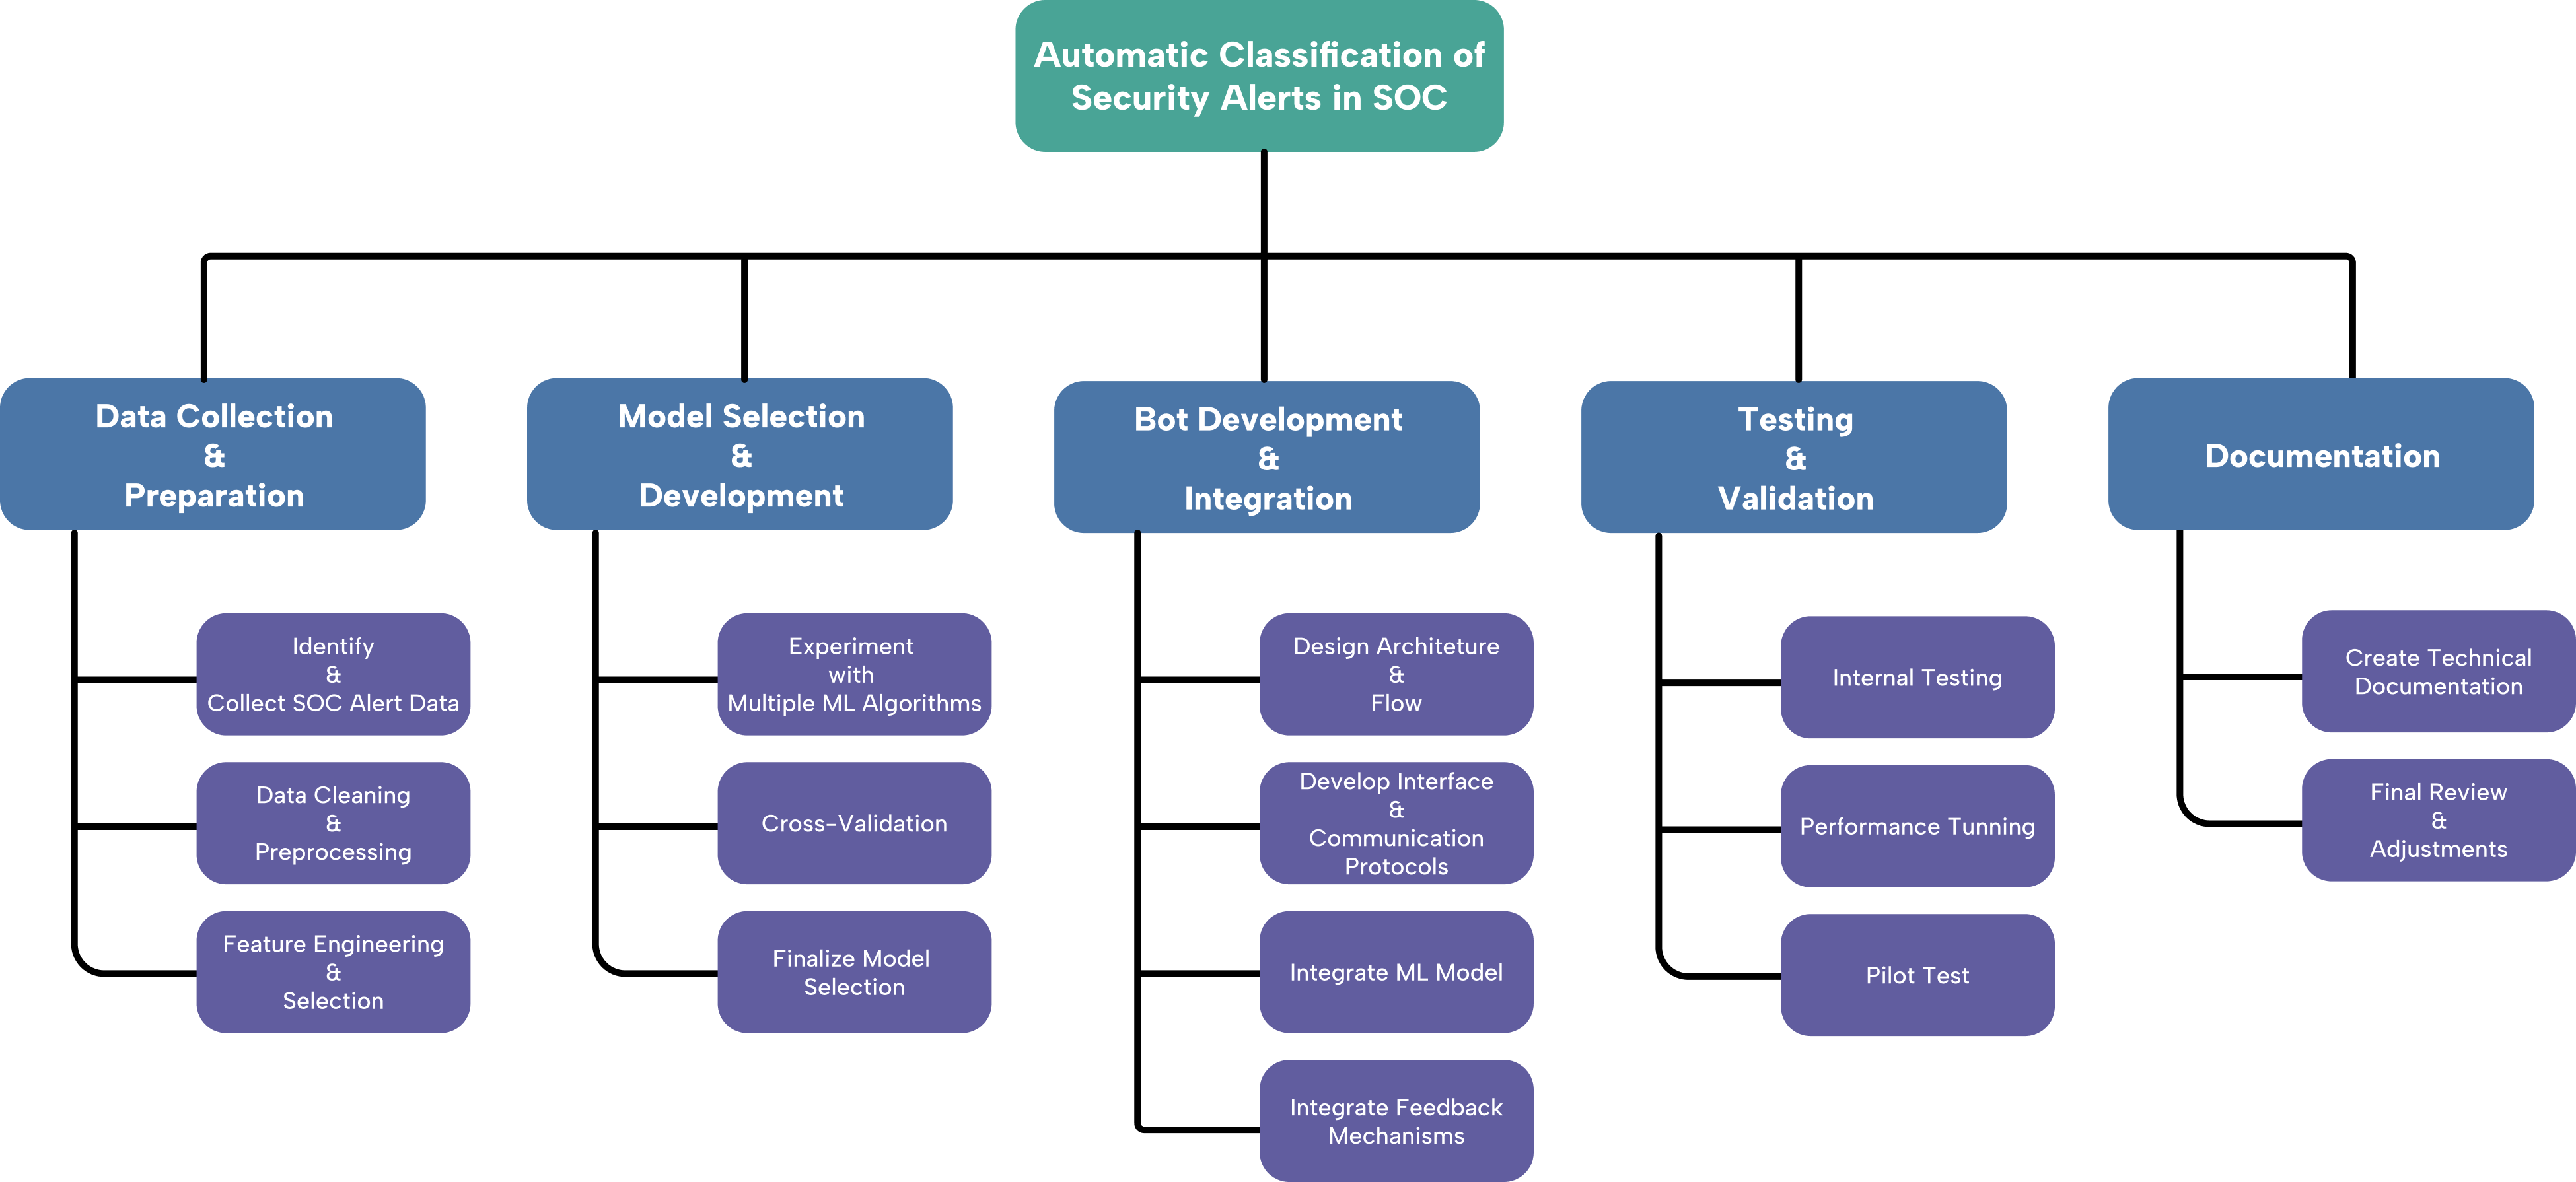
\includegraphics[scale=0.18, angle=270]{ch1/assets/WBS.png}
%     \caption{Work Breakdown Structure}
%     \label{fig:wbs-image} 
% \end{figure}

% \clearpage

%-------------------------------------------------------------------------------
\section{Dissertation Structure}

\textit{
    [ 
        Structure
    ]
}

%-------------------------------------------------------------------------------
%---------
%
% Chapter 2
\chapter{State of the Art}
\label{chap:Chapter2}

This chapter is divided into three parts. 
Part I starts on the theoretical side by introducing Machine Learning, Security Operation Centers, Security Information and Event Managers, and response mechanisms such as \gls{IPS}, \gls{IDS}, and \gls{EDR}. 
It also explains how popular \gls{ML} classification models work and how to evaluate them. 
Understanding these topics is the groundwork for material considered later in the chapter.

The second part focuses on the automatic classification of security alert tickets. 
It begins with an overview of proposed solutions and then reviews several publicly available studies. 
The chapter concludes with a detailed evaluation of existing systems that are similar to the one presented in this thesis. 

The third and final part discusses existing technologies that \gls{SOC} may utilize. 
These technologies are designed to support the workflow outlined in the first section about \gls{SOC}. 
At least three different technologies will be presented and discussed for each aspect of the \gls{SOC} workflow. 
The section will conclude with a summary of the key differences among the technologies and, if relevant, evaluate which one may be superior.

\section{Theoretical Introduction}

Before diving into the technologies, tools, and methodologies used for automating the classification of security alert tickets, it is essential to understand some fundamental concepts. 
Concepts like, \gls{SOC}s, \gls{SIEM} systems, \gls{AI}, particularly \gls{ML}, and advanced threat detection and response mechanisms. 
Such a foundation is indispensable for comprehending these systems' functions, construction work, advantages and limitations, and the actual performance comparison among different methods. 
The chapter introduces \gls{SOC} and how it functions, then moves on to the foundations of \gls{ML} and provides an overview of models frequently used for classification problems. 
It provides an overview of methods for assessing the performance of classification models, placing this in context for their use within the project.

\subsection{Security Operations Center} 

The complexity and frequency of cyber threats are increasing \parencite{Arianna2024}, which has led to the emergence of \gls{SOC}s as a critical component of modern IT enterprises. 
\gls{SOC}s are the primary defenders in incident response planning, vulnerability management, and regulatory compliance. 
In today's interconnected world, integrating security operations to reduce defensive barriers allows organizations to optimize resources, enhance security posture, and safeguard critical assets.

A \gls{SOC} is a unit \parencite{Rutledge2024} that provides tailored and centralized \gls{CND} \parencite{Zimmerman2014}. 
It defends computer networks against the growing world of cyber threats. 
The main objective of a \gls{SOC} is to ensure continuous monitoring and incident response for enterprise systems \parencite{Zimmerman2014}. 
This primarily focuses on preventing unauthorized access, cyber-attacks, and data breaches.

This \gls{24/7} facility leverages advanced technologies and skilled information security professionals to monitor the network continuously \parencite{Zimmerman2014}. 
With sophisticated tools to detect anomalies, a \gls{SOC} can address threats before they escalate.

\subsubsection{Definition and Characteristics of a SOC}
\textcite{Zimmerman2014} defined a \gls{SOC} as:
\begin{quote}
    ``A team primarily composed of security analysts organized to detect, analyze, respond to, report on, and prevent cybersecurity incidents.''
\end{quote}

This definition integrates elements from various sources, including the historical definition of \gls{CSIRT} as detailed in references \parencite{Shirey2007} and \parencite{Brownlee1998}. 

For an organization to qualify as a \gls{SOC}, according to \textcite{Zimmerman2014}, it must:
\begin{enumerate}
    \item Establish a system for constituents to report cybersecurity incidents.
    \item Provide comprehensive support for managing and resolving incidents effectively.
    \item Convey incident-related information to internal and external stakeholders.
\end{enumerate}

\subsubsection{Key Responsibilities of a SOC}
A \gls{SOC} has several critical missions, as outlined by various sources \parencite{Muniz2015, Zimmerman2014}:
\begin{itemize}
    \item Preventing cybersecurity incidents by implementing proactive measures such as vulnerability scanning and threat analysis.
    \item Monitor, detect, and analyze potential security intrusions.
    \item Handle confirmed incidents and coordinate resources for effective countermeasures.
    \item Providing stakeholders with situational awareness regarding cybersecurity incidents, trends, and threats.
\end{itemize}

\subsubsection{Tiers of Operation}
Analysts within a \gls{SOC} operate in tiers \parencite{Vielberth2020}. 
Tier 1 analysts monitor and conduct initial investigations, escalating complex cases to Tier 2 analysts, who perform in-depth analyses and take further actions like blocking activities or deactivating accounts. 
Generally, higher-tier analysts handle more complex incidents, which require more time to resolve.

\begin{figure}[ht]
    \centering
    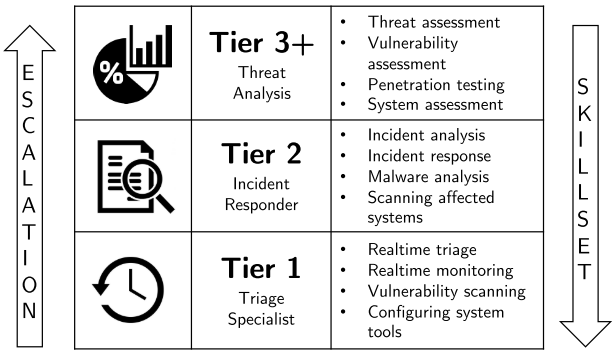
\includegraphics[width=\textwidth]{ch2/assets/tierTable.png}
    \caption{SOC Analyst Tier Responsibilities, from \autocite{Kokulu2019}.}
    \label{fig:soc-tier}
\end{figure}

Extra levels may exist that handle responsibilities like threat hunting, vulnerability assessments, and penetration testing. 
These levels are collectively termed Tier 3+. 
Figure~\ref{fig:soc-tier} was taken from a paper on a qualitative study on a \gls{SOC} \parencite{Kokulu2019} and illustrates a visual representation of these tiers and their associated tasks. 
Not all \gls{SOC}s follow a hierarchical model. 
In some collaborative frameworks, team members may possess comparable skill sets, enabling them to manage incidents independently \parencite{Kokulu2019}.

\subsubsection{Triage Specialist}

Since this project focuses on automating the triage process, it is crucial to gain a detailed understanding of the role of a triage specialist, their functions, and the advantages of automated triage in comparison.

Tier 1 analysts, also known as triage specialists, play a critical role in the initial stages of a \gls{SOC} workflow \parencite{Vielberth2020}. 

As stated by \textcite{Vielberth2020}, a Tier 1 analyst's primary responsibilities include:
\begin{enumerate}
    \item Collecting and analyzing raw data.
    \item Reviewing alarms and alerts generated by monitoring systems.
    \item Determining the validity and criticality of each alert.
\end{enumerate}

They must improve alerts with additional contextual information and decide whether an alert represents a real threat or a false positive \parencite{Hamornik2018, Sundaramurthy2014}. This process demands meticulous attention to detail, as the triage specialist must assess individual alerts, notify potential high-risk events, and prioritize them according to their severity \parencite{Tao2018}. 

The repetitive nature of triage work, coupled with the need to escalate unresolved issues to Tier 2 analysts, can result in mental fatigue and burnout \parencite{Tines2023, Iamnitchi2017}. This exhaustion affects individual performance and can compromise the overall efficiency of the \gls{SOC}, as delayed or missed alerts may result in critical threats going undetected \parencite{CriticalStart2019}.

In a 2018 study \parencite{Crowley2018}, 53\% of respondents in a security survey identified inadequate automation as the most common shortcoming.

This study demonstrates that effectively structured and implemented automation can help mitigate some or many of a \gls{SOC}'s weaknesses, particularly in the repetitive aspects of the \gls{SOC}'s workflow, such as the triage process.

\subsection{Security Information and Event Management}

The increasing complexity of cybersecurity threats has compelled organizations to implement advanced technologies to protect their digital assets. 
\gls{SIEM} systems have emerged as vital tools in this context \parencite{Shaw2022}.

\gls{SIEM} systems gather and centralize security-related data to detect threats and respond to incidents effectively. 
These systems connect logs from various sources to support security analytics, enabling real-time monitoring and retrospective analysis of past events \parencite{Shaw2022}.
They integrate with cyber threat intelligence platforms, providing human analysts with advanced visual tools for seamless information sharing between organizations. 
Additionally, they retain event data over extended periods, ensuring robust log management capabilities.

The key features of a \gls{SIEM} system, as gathered from various published sources \parencite{Harper2010, Sheeraz2023, Ali2024}, are:

\begin{itemize}
    \item \textbf{Log Collection:} SIEM gathers log data from various network devices such as servers, firewalls, and switches. Data can be collected using two methods:
    \begin{enumerate}
        \item \textbf{Agent-based collection:} An intermediary agent collects and forwards logs.
        \item \textbf{Agent-less collection:} Servers retrieve logs directly from the source devices.
    \end{enumerate}
    
    \item \textbf{Log Aggregation:} Collected logs are analyzed and structured for meaningful insights. Aggregation methods include:
    \begin{enumerate}
        \item \textbf{Push method:} Devices actively send logs to the SIEM.
        \item \textbf{Pull method:} SIEM retrieves logs as needed.
    \end{enumerate}
    
    \item \textbf{Parsing and Normalization:} Parsing converts raw logs into structured data, while normalization standardizes logs from diverse sources to eliminate redundancy.
    
    \item \textbf{Threat Analysis and Detection:} By correlating log data with known threat indicators, SIEM systems identify malicious activities. Statistical methods and predefined rules enhance their ability to detect sophisticated threats.
    
    \item \textbf{Response Automation:} SIEM systems issue real-time alerts and notifications, enabling rapid responses to potential incidents.
    
    \item \textbf{Reporting and Visualization:} Advanced reporting tools provide security analysts with actionable insights, enabling detailed investigations and trend analysis.
\end{itemize}

\subsubsection{Architectural Components}

The architectural components of a security information and Event Management (SIEM) system consist of several essential elements that enable effective security monitoring, incident detection, and response \parencite{Sheeraz2023}.

Data sources provide the raw material for analysis and threat detection \parencite{Ali2024}. These include a wide variety of log-generating devices and applications:
\begin{itemize}
    \item \textbf{Network devices}: Firewalls, routers, and switches.
    \item \textbf{Endpoint devices}: Workstations, servers, and mobile devices.
    \item \textbf{Applications}: Web servers, databases, and cloud platforms.
\end{itemize}

A variety of data sources is crucial for effective monitoring and threat detection. 

\textbf{Data collection} is a vital step with two main approaches to consider:
\begin{itemize}
    \item \textbf{Agent-based collection}: Agent-based collection uses proxy agents on endpoint devices for better control and flexibility in log collection, but it is costly and complex to manage.
    \item \textbf{Agent-less collection}: Agent-less collection allows devices to send data directly to the SIEM, simplifying deployment but may reduce efficiency in high-volume data environments.
\end{itemize}

The \textbf{SIEM processing engine} is one of the critical components \parencite{Sheeraz2023} responsible for:
\begin{itemize}
    \item \textbf{Parsing}: The conversion of raw log data into a structured format used for analysis.
    \item \textbf{Normalization}: Ensure the log formats are standardized to facilitate easier comparisons.
    \item \textbf{Correlation}: Finding relationships between events to strengthen security posture or incident response.
\end{itemize}

\textbf{Storage and rationalization} are vital for ensuring scalability and compliance. SIEM systems must store logs for future analysis.
This means there has to be enough storage and a logical way of organizing this data for scalability or compliance requirements like GDPR and HIPAA \parencite{Sheeraz2023}.
Effective storage solutions should scale dynamically to handle large datasets without compromising performance or compliance standards.

\textbf{Visualization and reporting tools} play a key role in making data accessible and actionable.
Critical functions that significantly benefit from good data visualization and reporting tools are incident investigation, trend analysis, and compliance audits \parencite{Sheeraz2023}. 
These features not only improve user experience but also aid in making data actionable and accessible. 
Organizations can use these tools to conduct incident investigations, identify patterns occurring over time, and monitor compliance \parencite{Sheeraz2023}. 
This comprehensive approach enables the development of scalable systems that can effectively handle increasing data demands.

\clearpage

\begin{figure}[ht]
    \centering
    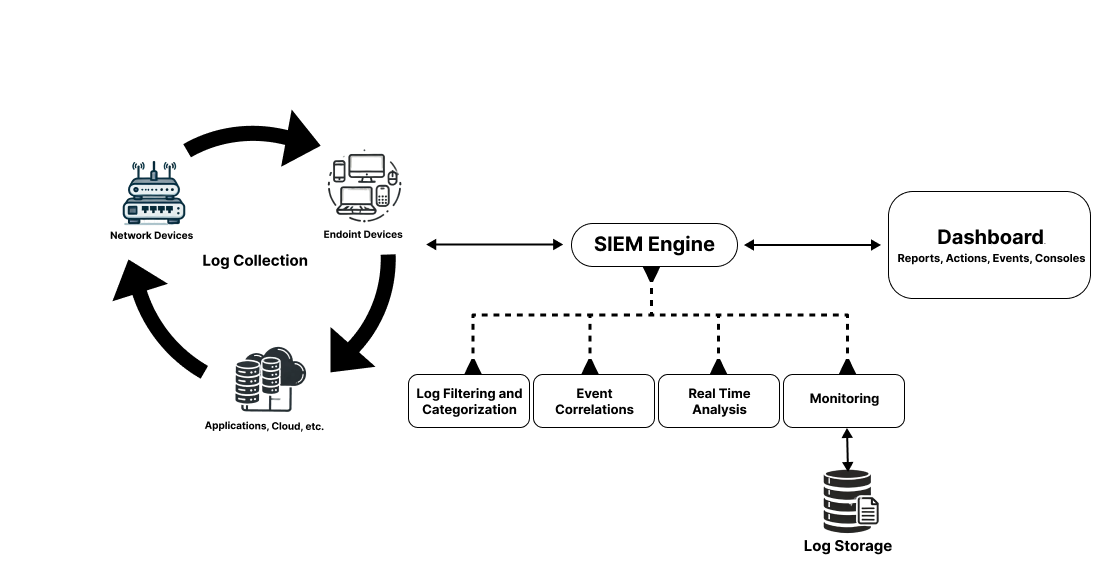
\includegraphics[width=\textwidth]{ch2/assets/FinalGraph.png}
    \caption{SIEM Architecture}
    \label{fig:siem-arc}
\end{figure}

Figure~\ref{fig:siem-arc} illustrates the architecture of a \gls{SIEM} system, highlighting its critical components and their interactions. 
Data flows from network and endpoint devices, as well as applications, to the log collection module. 
The \gls{SIEM} processing engine then parses, normalizes, and correlates this data for real-time security alert analysis, event monitoring, and threat detection.

The diagram also emphasizes the importance of visualization and reporting tools for turning data into actionable insights.

The graphic illustrates how these elements integrate into a SIEM.

\subsection{Machine Learning}

\gls{ML} is a core part of \gls{AI} but also overlaps with data mining, statistics, probability, and mathematics \parencite{Mohri2012}. 
Unlike traditional rule-based systems that rely on predefined logic, \gls{ML} uses induction—it learns patterns from past data and forms assumptions that can be generalized to new cases \parencite{Ali2024}. 
This method relies on datasets, which are groups of examples the \gls{ML} algorithm analyzes to find patterns \parencite{Mohri2012, Suthaharan2016}. 
The goal is to use these learned patterns to predict or describe new data.

There are three primary types of techniques employed in machine learning, \parencite{Mohri2012}:

\begin{enumerate}
    \item \textbf{Reinforcement Learning}: 
    This is a subset of machine learning in which an agent learns by interacting with the environment \parencite{Moradi2023}. It observes the environment, selects an action, and receives a reward if the action is beneficial or a penalty if it is detrimental. Over time, it refines its approach to achieve maximum rewards.

    \item \textbf{Supervised Learning}: 
    In this type of machine learning, models are trained on labeled data, meaning that each example includes input features and the corresponding expected output (or label). The model learns to map the inputs to the outputs, enabling it to predict the output for new, unseen data.

    \item \textbf{Unsupervised Learning}: 
    Unsupervised learning analyzes unlabeled data to reveal patterns without predefined labels. Unlike supervised learning, it allows algorithms to explore data independently. It is often used for clustering similar data points or modeling probability distributions. This approach is valuable for understanding the inherent organization in data without prior knowledge.
\end{enumerate}

Supervised learning can be further categorized into several types, \parencite{Mohri2012}:

\begin{itemize}
    \item \textbf{Regression}: 
    Regression algorithms predict numerical values within a continuous range by analyzing input data to identify patterns. They can forecast future values, such as calculating the next number in a sequence based on previous numbers and trends. Techniques like linear regression, polynomial regression, and others enable these algorithms to draw conclusions and make predictions effectively.
    
    \item \textbf{Similarity}: 
    Similarity algorithms analyze and compare two distinct instances to measure their resemblance. They are vital in recommender systems for suggesting products based on user preferences and in visual identity tracking and verification by comparing images or features. Their versatility makes them essential in data analysis, security, and personalized user experiences.
    
    \item \textbf{Classification}: 
    Classification algorithms classify the input data into predefined groups. Classification tasks can be binary when there are only two possible categories (such as a yes-no decision) or multiclass when the number of categories exceeds two, such as recognizing handwritten letters in the alphabet.
\end{itemize}

However, \gls{ML} has its limitations. 
Since datasets are finite, no algorithm can predict every scenario, which highlights an essential aspect of inductive reasoning: it can suggest likely outcomes but cannot ensure certainty \parencite{Mohri2012, Suthaharan2016}. 

In \gls{ML}, achieving an optimal model involves balancing between two critical concepts: \textbf{bias} and \textbf{variance}. 
Bias refers to the error introduced when a model is excessively simplistic, which can lead to underfitting. 
Underfitting occurs when the model fails to capture the underlying patterns of the data, resulting in poor performance on both training and unseen datasets \parencite{ElSahly2023}. 
On the other hand, variance arises when a model becomes overly complex and sensitive to the fluctuations in the training data, culminating in overfitting. 
Overfitting means the model performs exceptionally well on the training dataset but poorly on new, unseen data because it has memorized the noise instead of learning the actual signal \parencite{ElSahly2023}. 

The primary objective in constructing a machine learning model is to identify the appropriate level of complexity with the right balance, ensuring the model generalizes well and performs effectively on new data \parencite{Suthaharan2016}.

Despite these challenges, \gls{ML} continues to evolve, with increasingly sophisticated algorithms enabling breakthroughs in many fields \parencite{Mohri2012}. 

\subsection{Machine Learning Models}

The processes and computations of training a machine learning model are structured within a framework. 
This chapter will briefly overview the most frequently used algorithms relevant to this project's goals.

\subsubsection{Decision Trees}

Decision Trees (DTs) are a fundamental supervised machine learning algorithm for classification and regression tasks \parencite{Huang2024}. 
They work by splitting data into subsets based on the value of input features, forming a tree-like structure composed of nodes and branches.

The process begins at the root node, representing the entire dataset, and iteratively divides the data into homogeneous subsets using decision nodes until a terminal leaf node is reached, representing the output prediction or class \parencite{Chauhan2022}, as seen in Figure~\ref{fig:struc-DT}.

\begin{figure}[h]
    \centering
    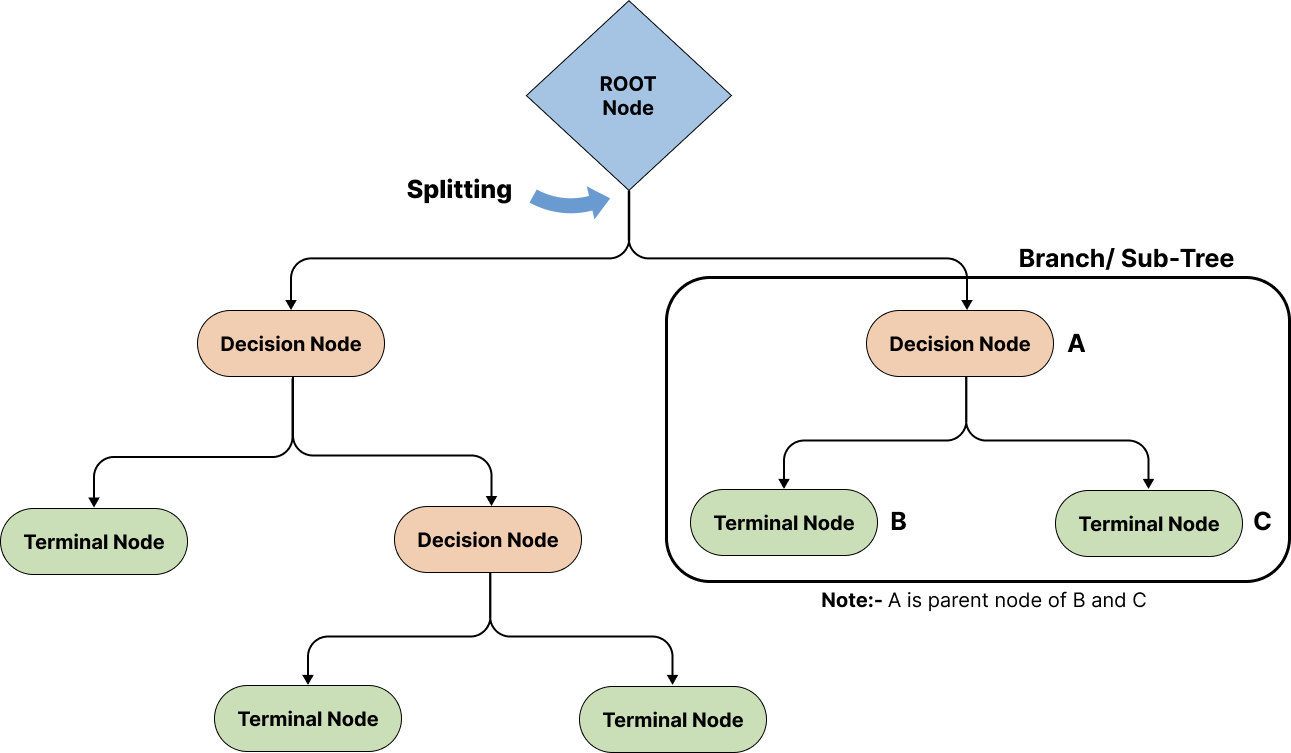
\includegraphics[width=\textwidth]{ch2/assets/FinalTreeGraph.png}
    \caption{A basic structure of a Decision Tree, based on \parencite{Chauhan2022}}
    \label{fig:struc-DT}
\end{figure}

The algorithm operates by evaluating all potential splits and selecting the one that optimizes a specific criterion, such as information gain or Gini impurity. 
Information gain measures the reduction in entropy after a split, while Gini impurity quantifies the likelihood of misclassification at a node. 

The entropy of \( S \) is defined as:
\begin{equation}
H(S) = \sum_{i=1}^{n} -P(s_i) \times \log_b P(s_i)
\end{equation}
where \( S \) is a set of values \( s_1, s_2, \dots, s_n \), \( P(s_i) \) is the probability of observing a certain value, and \( b \) is the logarithm base, most commonly \( 2 \), \( e \), or \( 10 \).

Using entropy, the \textbf{information gain (IG)} for a node \( t \) and a candidate split \( x \) is calculated as:
\begin{equation}
IG(t, x) = H(t) - H(x, t)
\end{equation}
In contrast, the \textbf{Gini index}, another commonly used metric for evaluating splits, is defined as:
\begin{equation}
\text{Gini} = 1 - \sum_{i=1}^{n} P(s_i).
\end{equation}

At each decision node, the algorithm tests a single feature and branches according to its value, guiding data instances down the tree until they reach a leaf node \parencite{Chauhan2022}. 
During training, the algorithm continues splitting until a stopping criterion is met, such as achieving a maximum tree depth, minimum node size, or no further improvement in the splitting metric \parencite{Chauhan2022}.

Pruning techniques prevent overfitting, which occurs when a tree becomes too complex and overly specific to the training data. 
These involve removing unnecessary branches or nodes to simplify the tree while maintaining predictive accuracy. 
Pruning can be preemptive (stopping tree growth early) or post hoc (removing branches after the tree is fully grown). 
This ensures that the decision tree generalizes well to unseen data \parencite{Huang2024}.

Decision trees are non-parametric, meaning they do not assume any specific distribution for the data, and they can capture both linear and non-linear relationships \parencite{Huang2024}. 
However, they are sensitive to slight variations in the dataset \parencite{Huang2024}, which may cause significant changes in the tree structure. 
Despite this, they remain popular for their simplicity, interpretability, and ability to handle numerical and categorical data \parencite{Chauhan2022}.

\subsubsection{Ensemble classifiers}

Ensemble learning is a powerful machine learning technique that combines the predictions of multiple base models to achieve superior performance compared to individual learners \parencite{Joseph2022}.

The fundamental idea is to address the limitations of single models, such as high variance, high bias, or low accuracy, by leveraging the diversity and complementary strengths of multiple models \parencite{Mienye2022, Dasarathy1979, Hansen1990}.

The concept of ensemble learning has evolved significantly since its inception. Early work by \textcite{Dasarathy1979} introduced the partitioning of feature spaces using multiple classifiers. 
Later, \textcite{Hansen1990} demonstrated that ensembles of artificial neural networks achieved superior predictive performance compared to single networks. 
\textcite{Schapire1990} groundbreaking work laid the foundation for boosting, one of the primary techniques in ensemble learning.

Ensemble learning methods are evaluated on two main principles: \textbf{accuracy} and \textbf{diversity} of the base learners \parencite{Hansen1990, Mienye2022}.

\begin{itemize}
    \item \textbf{Accuracy}: Each base learner should perform better than random guessing on the given task \parencite{Li2012}.
    \item \textbf{Diversity}: The errors made by individual learners should be uncorrelated, which can be achieved through techniques like subsampling, feature randomization, or algorithmic diversity \parencite{Schapire1990, Breiman1996}.
\end{itemize}

A model is accurate if it generalizes well on unseen instances, while diversity ensures that the errors of individual base models are not correlated. 
Achieving this balance is crucial for effective ensembles.

Ensemble Classifiers offer several advantages over single models, making them a popular choice in diverse applications of machine learning:
\begin{itemize}
    \item \textbf{Improved Generalization}: Ensembles reduce overfitting and improve generalization by aggregating the predictions of multiple learners \parencite{Hansen1990}.
    \item \textbf{Bias-Variance Trade-off}: Techniques like bagging reduce variance while boosting minimizes bias, addressing the critical limitations of individual learners \parencite{Li2012, Mienye2022}.
    \item \textbf{Adaptability}: Ensembles can be designed to work with homogeneous (same algorithm) or heterogeneous (different algorithms) base learners, making them versatile across domains \parencite{Mienye2022}.
\end{itemize}

Ensemble learning methods are broadly categorized into:
\begin{itemize}
    \item \textbf{Parallel Ensembles}: Base learners are trained independently on different subsets of data or features. Techniques like bagging and Random Forests fall into this category \parencite{Breiman1996}. The illustration in Figure~\ref{fig:parallel_emsemble} demonstrates how parallel ensembles operate.
    \item \textbf{Sequential Ensembles}: Models are trained iteratively, with each learner focusing on correcting the errors of its predecessor. Boosting is the most prominent example of this approach \parencite{Schapire1990}. The illustration in Figure~\ref{fig:sequential_emsemble} demonstrates how sequential ensembles operate.
    \item \textbf{Stacked Ensembles}: Predictions from multiple base models are combined using a meta-model trained on the outputs of the base learners \parencite{Mienye2022}.
\end{itemize}

\begin{figure}[b!]
    \centering
    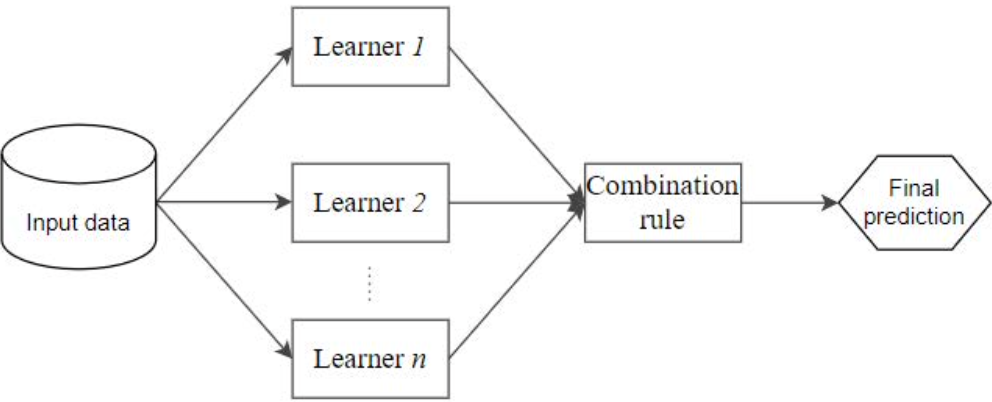
\includegraphics[width=\textwidth]{ch2/assets/Block_diagram_of_parallel_ensemble_learning.png}
    \caption{Diagram of Parallel Ensemble Learning from \parencite{Mienye2022}}
    \label{fig:parallel_emsemble}
\end{figure}

\clearpage

\begin{figure}[t!]
    \centering
    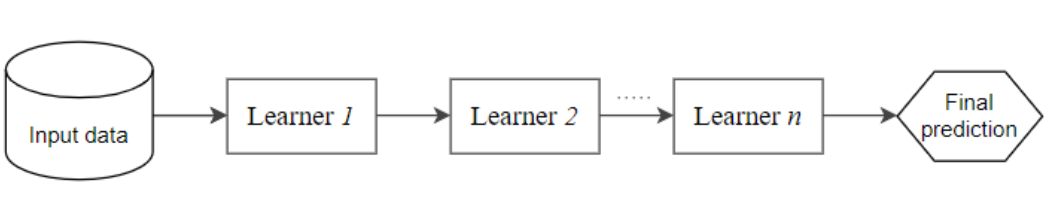
\includegraphics[width=\textwidth]{ch2/assets/Block_diagram_of_sequential_ensemble_learning.png}
    \caption{Diagram of Sequential Ensemble Learning. from \parencite{Mienye2022}}
    \label{fig:sequential_emsemble}
\end{figure}

Ensemble methods can then be categorized into three main approaches based on how they train and combine base models: \textbf{Bagging}, \textbf{Boosting}, and \textbf{Stacking}. 
Each method has a distinct mechanism for generating diversity and aggregating predictions, addressing the specific limitations of single models.

\paragraph{Bagging}
Bagging, which stands for bootstrap aggregating, is a parallel ensemble technique where multiple base models are independently trained on random subsets of the training data, referred to as bootstrapped samples. 
The final predictions are made by aggregating the outputs of these models, often using majority voting or averaging. 
Random Forests are a well-known implementation of bagging, recognized for their ability to reduce variance without increasing bias \parencite{Mienye2022}.

\paragraph{Boosting}
Boosting is a sequential ensemble method that aims to reduce bias by iteratively training base models. 
Each subsequent model focuses on correcting the errors made by the previous one, assigning higher weights to misclassified samples. 
Algorithms such as AdaBoost and Gradient Boosting exemplify this approach, often achieving superior performance on complex datasets, but this can lead to increased susceptibility to overfitting \parencite{Mienye2022}.

\paragraph{Stacking}
Stacking integrates predictions from multiple base models using a meta-model that learns the optimal way to combine their outputs. 
Unlike bagging and boosting, stacking allows for heterogeneous base learners, providing greater flexibility and diversity. 
The meta-model is typically trained on the predictions made by the base models, enabling it to make more accurate decisions \parencite{Mienye2022}.

\subsubsection{Random Forests}

Random Forests represent a significant advancement in machine learning, particularly in the domain of ensemble classifiers \parencite{Ali2024}. 

As a bagging-based ensemble method, Random Forests combine multiple decision trees to improve classification accuracy and robustness. 
This approach leverages the strengths of individual trees while mitigating their limitations, such as overfitting, by aggregating their predictions \parencite{Ali2024}. 

The Random Forest algorithm begins by generating multiple decision trees, as can be seen on Figure~\ref{fig:random_forest_algorithm}, each trained on a random subset of the training data through bootstrapping\footnote{Bootstrapping is a resampling technique where random samples are drawn with replacement from the dataset.}.
Additionally, features are randomly sampled at each split to ensure diversity among the trees, a process that reduces the correlation between individual tree predictions \parencite{Farooq2018}. 
Once trained, the predictions of all trees are aggregated, typically through majority voting for classification tasks or averaging for regression tasks, to produce the final output \parencite{Nila2020}. 

\begin{figure}[h!]
    \centering
    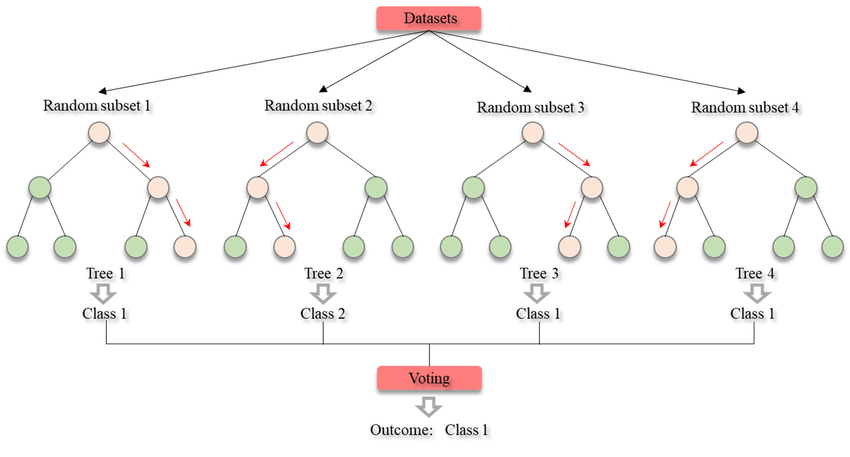
\includegraphics[width=\textwidth]{ch2/assets/Workflow-of-the-random-forest-algorithm.ppm.png}
    \caption{Workflow of Random Forests: Bootstrapping, Decision Trees, and Aggregated Predictions from \parencite{Yang2019}}
    \label{fig:random_forest_algorithm}
\end{figure}

Random Forests are highly valued for their versatility and robustness. 
They perform exceptionally well with large and high-dimensional datasets, effectively handling numerical and categorical data. 
Furthermore, their inherent ability to measure feature importance makes them interpretable, a critical requirement in security domains where trust and explanation are essential \parencite{Ali2024}. 

Random Forests also excel at reducing overfitting, a common issue with individual decision trees. 
By averaging the predictions of multiple trees, the model achieves better generalization, even when faced with noisy data \parencite{Sopan2019}. 

Random Forests have been widely adopted in cybersecurity applications, particularly for detecting anomalies, classifying alerts, and predicting the likelihood of malicious behavior. 
For example, they are effectively used in \gls{SIEM} systems to process large volumes of log data, identify patterns, and reduce false positives \parencite{Farooq2018, Ali2024}. 

Studies have shown that Random Forest-based models can achieve high accuracy in detecting advanced persistent threats (APTs) and other cyberattacks by leveraging their ability to handle complex feature interactions and high-dimensional data \parencite{Ali2024}. 
For instance, combining Random Forests with additional modules for feature selection and preprocessing has improved detection rates and reduced manual intervention in incident response workflows \parencite{Nila2020}.

\subsubsection{Naive Bayes}

The Naive Bayes algorithm is a probabilistic classifier based on Bayes' theorem, which assumes conditional independence among features given the class \parencite{Chandra2016}.
This simplicity makes it computationally efficient and easy to implement. 

Naive Bayes is particularly effective in scenarios where the assumption of feature independence is approximately attained, such as spam detection and document classification. 
The model's reliance on this assumption allows it to scale effectively to high-dimensional datasets while remaining computationally efficient \parencite{Chandra2016}.

Naive Bayes calculates the posterior probability of each class given the observed data using the formula:

\begin{equation}
P(C|X) = \frac{P(X|C) \cdot P(C)}{P(X)}
\end{equation}

where:
\begin{itemize}
    \item \( P(C|X) \) is the posterior probability of class \( C \) given the feature vector \( X \),
    \item \( P(X|C) \) is the likelihood of observing \( X \) given class \( C \),
    \item \( P(C) \) is the prior probability of class \( C \),
    \item \( P(X) \) is the probability of the feature vector \( X \).
\end{itemize}

In practice, the Naive Bayes model, Figure~\ref{fig:naive_bayes}, estimates the prior probability \( P(C) \) for each class and the conditional probability \( P(X_i|C) \) for each feature \( X_i \) given the class. 
These probabilities are typically derived from the frequency of occurrences in the training data. 
For continuous features, it is common to assume a Gaussian distribution and compute the likelihood accordingly. 
The model assigns a new instance to the class with the highest posterior probability \( P(C|X) \) \parencite{Nila2020, Chandra2016}.

\begin{figure}[h!]
    \centering
    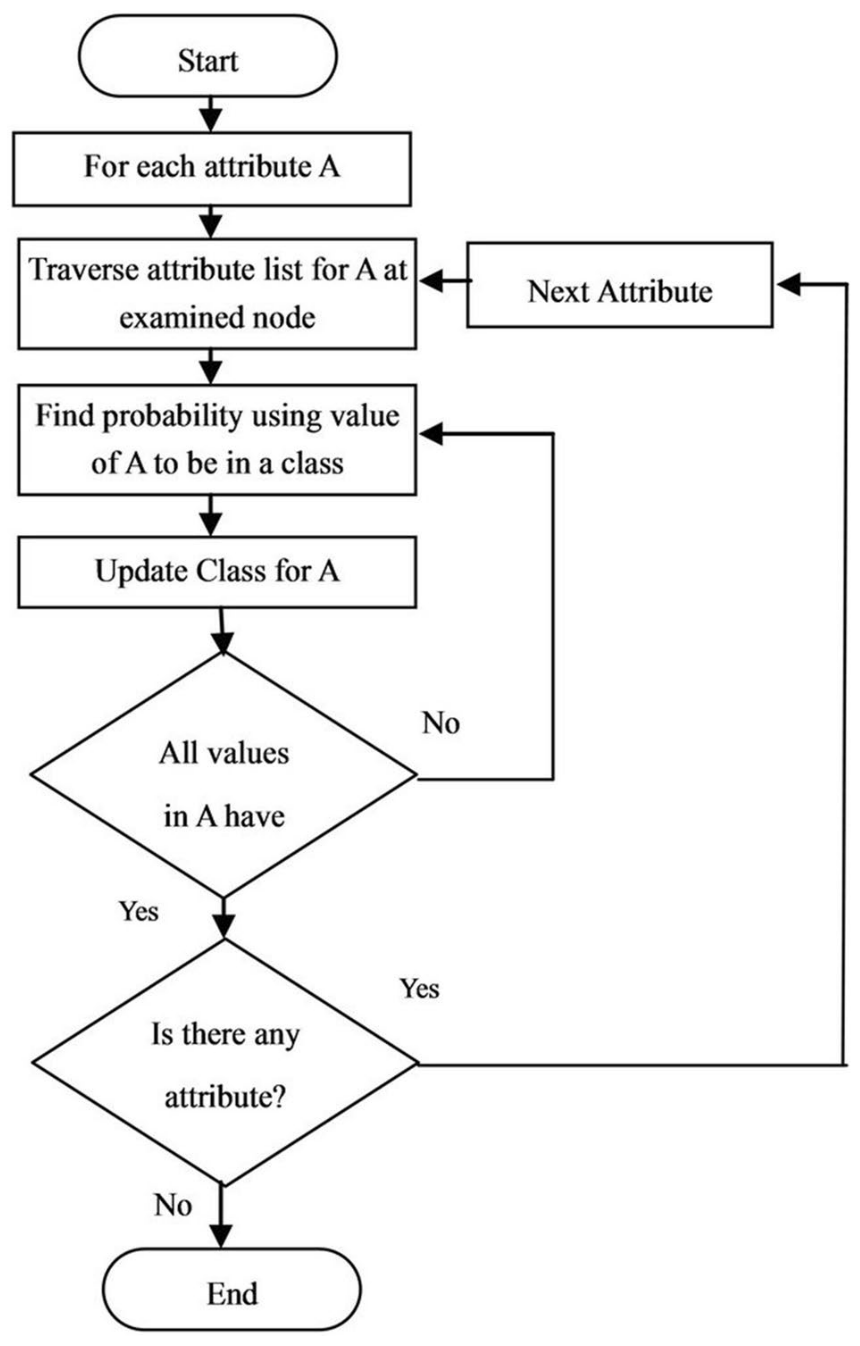
\includegraphics[width=0.3\textwidth]{ch2/assets/Flow-chart-for-Naive-Bayesian-classification.png}
    \caption{Schematic Diagram of the Naive Bayes Classification Process from \parencite{Sneha2019}}
    \label{fig:naive_bayes}
\end{figure}

This decision rule is computationally efficient, making Naive Bayes suitable for real-time prediction tasks \parencite{Nila2020, Chandra2016}. 

However, the strong independence assumption may only hold in some scenarios, potentially leading to suboptimal performance when features are highly correlated. 
Despite this limitation, Naive Bayes remains popular due to its simplicity and effectiveness in many practical applications \parencite{Chandra2016}.

\section{Automatic Classification of Security Alerts in SOC}

The growing complexity of cyber threats, especially \gls{APT}, has led to significant advancements in automated detection and mitigation mechanisms. 
Many of these mechanisms utilize \gls{ML} techniques. 
This section examines key works, focusing on their methodologies, limitations, and relevance to the problem of alert triage automation in \gls{SOC}.

Recent research has explored hybrid approaches to anomaly detection. 
\textcite{Saini2023} proposed a hybrid ensemble model combining Random Forest and XGBoost classifiers, achieving a 99.91\% accuracy on the CIC-IDS2017\footnote{Labeled dataset of network traffic, including normal behavior and various attacks, used to evaluate intrusion detection models.} dataset with a False Positive Rate (FPR) as low as 0.12\%. 
Despite its high performance, the model relies on static datasets, which limits its adaptability to evolving attack patterns. 
Similarly, \textcite{Ghafir2018} developed Machine Learning for Advanced Persistent Threats (MLAPT), a multi-phase system incorporating correlation frameworks for APT detection, achieving an accuracy of 84.8\%. 
While this approach improved early-stage prediction, its accuracy was limited compared to ensemble methods and lacked scalability for dynamic environments.

\textcite{Ali2024} extended APT datasets to include a diverse range of alerts. 
They integrated Random Forest and XGBoost models into a SIEM environment, demonstrating the ability to reduce FPR and achieve a near-perfect 99.6\% accuracy. 
However, the computational demands of such systems may hinder practical deployment in resource-constrained environments.
On the contrary, \textcite{Brogi2016} utilized Information Flow Tracking (IFT) for APT detection, concentrating on the correlation between the various stages of an attack. 
While this method excels at tracing complex multi-stage attacks, it requires further automation to support large-scale SOC operations effectively.

Incorporating reinforcement learning, \textcite{Sethi2020} introduced a Deep Q-Network (DQN)-based context-adaptive intrusion detection system, which improved FPR and demonstrated robustness against several attacks. 
Nevertheless, the distributed nature of their approach introduces practical deployment challenges, especially in SOC environments where centralized oversight is critical. 
Similarly, \textcite{Nila2020} explored ML-based triage systems to automate alert classification and reduce false positives. 
Their work effectively alleviated analyst fatigue by prioritizing actionable alerts, yet the scope of implementation remains limited to standalone systems.

\textcite{Chandra2016} conducted a comprehensive study on email-based APT entry points, explicitly exploring the effectiveness of Bayesian spam filters\footnote{Bayesian spam filters classify emails as spam or legitimate using probabilities based on Bayes theorem.}.
These filters demonstrated a strong capability to identify and differentiate between spear-phishing attempts and general spam emails, which is crucial for enhancing cybersecurity measures. 
However, the authors noted that while their solution provided significant benefits in detecting these specific types of email threats, it needed to address the broader range of APT life cycles.
This limitation restricts its effectiveness in SOC environments with diverse attack vectors, requiring a more holistic approach to threat detection and response strategies to encompass the full spectrum of APT strategies and tactics.

Table~\ref{tab:related_work_table} presents a detailed summary of the relevant studies explored, highlighting their respective strengths, weaknesses, and potential areas for enhancement.

\captionsetup[table]{font=small} % Set the caption font size
\scriptsize % Reduce the font size for the table content
\begin{longtable}{@{}P{1.9cm}P{1.9cm}P{1.9cm}P{1.9cm}P{1.9cm}P{3cm}@{}}
    \caption{Summary of the Existing Related Works based on \textcite{Ali2024}.}
    \label{tab:related_work_table} \\
    \toprule
    \textbf{References} & APT Life Cycle Coverage & AI Models Used & Lowest FPR & Highest Accuracy & Limitations \\
    \midrule
    \endfirsthead
    \toprule
    \textbf{References} & APT Life Cycle Coverage & AI Models Used & Lowest FPR & Highest Accuracy & Limitations \\
    \midrule
    \endhead
    \bottomrule
    \endfoot
    \bottomrule
    \endlastfoot
    \textcite{Ghafir2018} & Complete & Decision Tree, SVM, KNN, Ensemble Classifier & 4.5\% & 84.8\% & The blacklist-based detection modules require continuous update. Moreover, the accuracy is lower. \\
    \hline
    \textcite{Brogi2016} & Complete & No ML model used & High & Not calculated & Information Flow Tracking is used to detect APTs; however, the FPR is high. \\
    \hline
    \textcite{Giura2012} & Complete & No ML model used & 27.88\% & Not calculated & Sufficient knowledge is required to set up the mechanism. \\
    \hline
    \textcite{Sopan2019} & No & Random Forest & Not calculated & 98.5\% & The post-alert decision is not automated; it involves the intervention of security experts. \\
    \hline
    \textcite{Farooq2018} & Partial & SVM, Random Forest & Not calculated & Not calculated & The process anomaly detection is presented formally using One-Class SVM. However, the paper lacks ML-based experimental results. \\
    \hline
    \textcite{Sethi2020} & No & Deep Q-network & 0.35\% & 96.12\% & The proposed model enables the detection of APTs. \\
    \hline
    \textcite{Nila2020} & No & ZeroR, OneR, NaiveBayes, SVM, J48, RandomForest & Not calculated & 95.5\% & The authors did not discuss the FPR of the proposed model. \\
    \hline
    \textcite{Chandra2016} & Partial & NaiveBayes & Not calculated & 87\% & The authors did not discuss the FPR of the proposed model. \\
    \hline
    \textcite{Saini2023} & Partial & Random Forest, XGBoost & 0.12\% & 99.91\% & This study used existing datasets, posing a challenge because these datasets might not contain the latest attack scenarios. \\
    \hline
    \textcite{Ali2024} & Complete & Random Forest, XGBoost & Not calculated\% & 99.6\% & High resource demand for training; dataset generated in controlled environments, limiting real-world adaptability. \\
\end{longtable}

\normalsize

This study introduces a new approach to automating alert triage in SOCs by combining ML models with existing SIEM systems. 
In contrast with the previous studies, this research will use live data as its training data and will be deployed in a real-world environment. 
Therefore, analysts can focus on high-risk issues by analyzing the alerts based on the severity of the cyber threat shown by the ML model.

While the related works reviewed in this study showcase significant advancements in SOC automation and alert triage, none closely reflects this research's objectives. 
However, beyond academic research, commercially available solutions like Check Point's SOC automation tools demonstrate functionalities that align with aspects of this study. 
These solutions offer valuable insights into the application of AI and automation in SOC environments, providing a practical point of comparison for the approach proposed in this research.

Check Point's approach to SOC automation stands out for its focus on streamlining SOC operations using artificial intelligence (AI) and automation tools \parencite{checkpoint}.

SOC automation, as described by Check Point, employs AI to take over repetitive and manual tasks in the SOC, such as alert triage, incident response, and threat detection. Their solution includes tools like:
\begin{itemize}
    \item \textbf{Generative AI:} Used to improve usability and streamline workflows, enabling analysts to query and interact with data using natural language.
    \item \textbf{Playbooks:} Predefined and customizable workflows for incident response that enable rapid and consistent remediation.
    \item \textbf{Threat Detection and Analytics:} Leveraging advanced analytics, behavioral insights, and proprietary threat intelligence from Check Point Research and ThreatCloud AI to identify threats and reduce false positives.
    \item \textbf{Malware Analysis and Phishing Detection:} Using sandboxes and natural language processing (NLP) to analyze suspicious files and emails.
    \item \textbf{Infinity Extended Prevention and Response (XDR/XPR):} A platform that integrates automated playbooks with real-time threat intelligence and analytics to correlate events across the security estate, detect sophisticated attacks, and prevent lateral movement.
\end{itemize}

The research in this study aligns closely with Check Point’s SOC automation approach. 
Both aim to automate alert triage and streamline SOC operations using AI to enhance efficiency. 
This study also shares key goals, such as reducing false positives, prioritizing alerts, and providing analysts with tools to focus on high-risk threats. 
Like Check Point, this research emphasizes the use of playbooks for consistent responses and aims to alleviate the burden of repetitive tasks on analysts.

While the Check Point solution is comprehensive and includes a full suite of tools, this research focuses on a customized solution tailored to the specific needs of the organization conducting this study differing in:
\begin{enumerate}
    \item \textbf{Integration with Existing Infrastructure:} This study develops a solution that seamlessly integrates with the organization's current SIEM system, avoiding the need for a complete overhaul of existing systems, as would be required to adopt Check Point’s platform.
    \item \textbf{Live Data and Real-World Deployment:} Unlike Check Point’s reliance on proprietary threat intelligence and prebuilt systems, this research involves using live data collected within the organization's environment, ensuring the model is trained and deployed in a real-world context.
\end{enumerate}

\section{Technologies}


The following section presents some of the important technologies available in the three categories discussed: SIEM Tools, Ticketing Tools, and Machine Learning Frameworks. 
The company utilizes QRadar as its SIEM solution and IBM QRadar SOAR and JIRA for ticketing and incident management. The subsequent subsections provide an overview of the tools in each category, followed by a comparative analysis highlighting their strengths and trade-offs.


The following section presents some of the important technologies available in the three categories discussed: SIEM Tools, Ticketing Tools, and Machine Learning Frameworks. 
Each category serves a unique purpose in the automatic classification of security alerts in a SOC.
The tools used for this project were the same as those the company utilizes, including QRadar as its SIEM solution, IBM QRadar SOAR, and JIRA for ticketing and incident management.
The subsequent subsections provide an overview of existing tools in each category, followed by a comparative analysis highlighting their strengths and trade-offs.

\subsection{SIEM Tools}

In this subsection, the three leading SIEM tools, QRadar, Splunk, and LogRhythm \parencite{exabeam2024}, were chosen for their advanced threat detection, log aggregation, and real-time security analytics. 
Based on industry adoption, integration capabilities, and performance in SOC environments, each platform offers unique features for efficient incident detection and response.

\subsubsection{QRadar}
QRadar is a SIEM solution initially developed by IBM and later acquired by Palo Alto Networks \parencite{paloalto2024}. 
It excels in advanced threat detection, log aggregation, and automated incident response by collecting and correlating data from various sources like firewalls and network devices. Its features, including anomaly detection and event prioritization, help analysts focus on critical threats, reducing false positives.

A key advantage of QRadar is its integration with other IBM and Palo Alto tools, facilitating seamless workflows. 
Its machine learning support enables organizations to detect emerging threats, while its modular architecture ensures scalability for businesses of all sizes. 
Recent updates enhance QRadar's capabilities for modern hybrid and cloud-native infrastructures.

\subsubsection{Splunk}
Splunk is a powerful and versatile SIEM platform known for its real-time monitoring and analytics. 
It enables organizations to detect and respond to cybersecurity threats quickly. 
It excels at processing large volumes of machine-generated data, making it essential for security teams in complex IT environments.

With a broad ecosystem of applications, Splunk supports various use cases such as threat hunting, compliance management, and anomaly detection. 
Splunk Enterprise Security (ES)'s add-on offers tailored solutions for SOC environments, including prebuilt dashboards and customizable alerts. 

Splunk's user-friendly interface and robust reporting tools cater to analysts of all skill levels, while its integration with machine learning enhances proactive threat management. 
Splunk's flexibility and capabilities make it a preferred choice for organizations seeking a reliable SIEM solution.

\subsubsection{LogRhythm}
LogRhythm is a robust SIEM platform aimed at enhancing threat detection and incident response. 
Its user-friendly design and integration capabilities help streamline SOC workflows. 
The platform utilizes advanced analytics, behavioral anomaly detection, and machine learning for effective threat identification. 

LogRhythm also excels in compliance management with preconfigured templates for regulations like GDPR, HIPAA, and PCI-DSS. 
Its Threat Lifecycle Management (TLM) framework facilitates efficient threat detection and remediation with structured workflows. 

A key highlight is its seamless integration with various third-party tools, along with a centralized dashboard that provides actionable insights for SOC teams. 
Additionally, LogRhythm offers flexible deployment options, making it suitable for diverse infrastructure needs.

\subsection{Ticketing Tools}

This subsection focuses on three ticketing tools: IBM QRadar SOAR, ServiceNow, and JIRA. 
These tools were selected for their capabilities in automating workflows, improving incident management, and integrating with \gls{SIEM} systems. 
Practical ticketing tools are vital for efficiently managing security incidents, reducing response times, and promoting collaboration within \gls{SOC} teams.

\subsubsection{IBM QRadar SOAR}
IBM QRadar SOAR enhances the QRadar SIEM platform by streamlining incident management and security operations. 
It automates workflows, minimizing manual tasks, and features playbook automation that allows analysts to execute consistent responses tailored to organizational policies. 
The comprehensive case management system centralizes tracking of incidents, evidence, and communications, fostering real-time collaboration. 
Additionally, it integrates with various third-party tools like EDR systems and cloud services, enabling SOC teams to focus on high-priority threats and improving overall efficiency in incident resolution \parencite{ibm}.

\subsubsection{ServiceNow}
ServiceNow is a versatile platform originally designed for IT service management (ITSM) that has expanded to include strong incident management for cybersecurity. 
It is widely adopted across industries and integrates effectively with SIEM tools and other security systems, making it valuable for SOC teams.

The Security Incident Response (SIR) module offers a centralized approach for managing security incidents, featuring workflow automation for incident triage, escalation, and remediation. 
Its dashboard capabilities enable real-time monitoring and reporting, providing security managers with visibility into ongoing incidents.

A key strength of ServiceNow is its seamless integration with vulnerability scanners, endpoint protection platforms, and threat intelligence feeds, enhancing its ability to prioritize alerts and correlate events. 
Its scalable architecture makes it suitable for organizations of all sizes, from small businesses to global enterprises.

\subsubsection{JIRA}
JIRA is widely recognized as a project management tool and has been adapted to manage security incidents in SOC environments. 
Its user-friendly interface allows organizations to enhance incident management with minimal training requirements. 
JIRA's ticketing system helps analysts create, assign, and update tickets for security alerts, ensuring systematic documentation and resolution.

JIRA integrates effectively with SIEM tools and offers extensive customization options for workflows and notifications, further enhancing its functionality. 
Although it lacks advanced features like playbook-driven automation found in IBM QRadar SOAR, JIRA remains a practical and cost-effective solution for incident management, especially for organizations already familiar with its ecosystem.

\subsection{Machine Learning Frameworks}

This section discusses three popular machine learning frameworks: Scikit-learn, TensorFlow, and PyTorch \parencite{mlframeworks}.
These frameworks effectively implement scalable machine learning models in research and production. 

\subsubsection{Scikit-learn}
Scikit-learn is a Python library known for its simplicity in implementing classical machine learning algorithms like Random Forest, Naive Bayes, and Support Vector Machines (SVM). 
It excels in classification, regression, and clustering tasks and offers comprehensive preprocessing tools for effective data cleaning and transformation. 
The library features strong cross-validation capabilities for evaluating model performance and integrates well with other Python libraries such as NumPy, pandas, and matplotlib. Scikit-learn is ideal for quick prototyping and development, making it a popular choice for both beginners and professionals, though it may not be as effective for deep learning or very large datasets.

\subsubsection{TensorFlow}
TensorFlow is an open-source framework developed by Google, designed for scalable machine learning and deep learning applications. 
It efficiently handles large-scale computations and supports various techniques, including traditional algorithms and advanced architectures like CNNs and RNNs. 
The Keras API within TensorFlow simplifies model building for users with limited experience.

One of its key strengths is deploying models across platforms like mobile, edge computing, and cloud environments. 
TensorBoard, a visualization tool, helps users monitor training and performance, enabling effective algorithm fine-tuning. 
Despite a steeper learning curve compared to some alternatives, TensorFlow's extensive capabilities make it ideal for complex applications, including cybersecurity tasks like anomaly detection and threat prediction.

\subsubsection{PyTorch}
PyTorch is a flexible machine learning library that has gained popularity among researchers and developers due to its dynamic computation graph, allowing real-time changes during model execution. 
It excels in deep learning tasks like natural language processing, computer vision, and reinforcement learning, with the torch.nn module simplifying neural network creation and the autograd module providing efficient gradient computation. 
PyTorch's intuitive design makes it easy for new users and integrates well with libraries like NumPy and ONNX. 

\subsection{Comparative Analysis}

A comparative overview of all the discussed technologies will be presented here. This analysis highlights the strengths and limitations of the SIEM tools, ticketing tools, and machine learning frameworks identified in previous subsections.

\subsubsection{SIEM Tools}

\begin{longtable}{p{3cm}p{3cm}p{3cm}p{3cm}}
    \caption{Comparative Analysis of SIEM Tools.}
    \label{tab:siem_ca} \\
    \toprule
    \textbf{Feature} & \textbf{QRadar} & \textbf{Splunk} & \textbf{LogRhythm} \\
    \midrule
    \endfirsthead
    \toprule
    \textbf{Feature} & \textbf{QRadar} & \textbf{Splunk} & \textbf{LogRhythm} \\
    \midrule
    \endhead
    \bottomrule
    \endfoot
    \bottomrule
    \endlastfoot
    Integration & Deep IBM ecosystem integration & Extensive third-party support & Moderate third-party support \\
    Threat Detection & Advanced anomaly detection & Real-time search and analytics & Strong ML-based detection \\
    Compliance & Strong compliance capabilities & Flexible for custom compliance & Focused on compliance workflows \\
    Machine Learning & Limited native ML & Third-party ML integrations & Native ML capabilities \\
    Ease of Use & Moderate & User-friendly UI & Moderate \\
\end{longtable}

As shown in Table~\ref{tab:siem_ca}, QRadar stands out due to its deep integration with IBM solutions, making it an excellent choice for organizations already utilizing IBM's ecosystem. 
In contrast, Splunk offers powerful real-time analytics and extensive integration with third-party tools, which allows it to be adaptable for various use cases. 
LogRhythm focuses on compliance and features native machine learning capabilities, although it may not provide the same level of seamless integration within IBM environments as QRadar does.

\clearpage

\subsubsection{Ticketing Tools}

\begin{longtable}{@{}p{3cm}p{3cm}p{3cm}p{3cm}@{}}
    \caption{Comparative Analysis of Ticketing Tools.}
    \label{tab:tt_ca} \\
    \toprule
    \textbf{Feature} & \textbf{QRadar SOAR} & \textbf{ServiceNow} & \textbf{JIRA} \\
    \midrule
    \endfirsthead
    \toprule
    \textbf{Feature} & \textbf{IBM QRadar SOAR} & \textbf{ServiceNow} & \textbf{JIRA} \\
    \midrule
    \endhead
    \bottomrule
    \endfoot
    \bottomrule
    \endlastfoot
    Integration & Seamless with QRadar SIEM & Broad integrations across IT & Extensive integrations with development tools \\
    Automation & Playbook-driven workflows & Customizable workflow automation & Moderate workflow automation \\
    Incident Management & Case management and playbooks & Advanced IT service management & Simplified incident tracking \\
    Ease of Use & Moderate & Customizable but complex & Highly user-friendly \\
\end{longtable}
    
Table~\ref{tab:tt_ca} outlines the strengths and weaknesses of various ticketing tools. 
IBM QRadar SOAR closely integrates with the QRadar SIEM platform, providing strong automation through playbooks and advanced incident management features. 
ServiceNow is notable for its flexibility and capability to cater to multiple IT departments. 
In contrast, JIRA offers a more user-friendly and cost-effective solution, with moderate automation functionalities and extensive integration capabilities.

\subsubsection{Machine Learning Frameworks}

\begin{longtable}{@{}p{3cm}p{3cm}p{3cm}p{3cm}@{}}
    \caption{Comparative Analysis of Machine Learning Frameworks.}
    \label{tab:ml_ca} \\
    \toprule
    \textbf{Feature} & \textbf{Scikit-learn} & \textbf{TensorFlow} & \textbf{PyTorch} \\
    \midrule
    \endfirsthead
    \toprule
    \textbf{Feature} & \textbf{Scikit-learn} & \textbf{TensorFlow} & \textbf{PyTorch} \\
    \midrule
    \endhead
    \bottomrule
    \endfoot
    \bottomrule
    \endlastfoot
    Algorithms Supported & Classical ML (Random Forest) & Deep Learning and Classical ML & Deep Learning and Research ML \\
    Scalability & Moderate & High & High \\
    Ease of Use & Beginner-friendly & Moderate complexity & High flexibility for research \\
    Deployment & Less optimized for deployment & Production-ready & Suitable for research \& testing \\
    Flexibility & Limited to classical models & High for both models and tuning & High for experimentation \\
\end{longtable}

As outlined in Table~\ref{tab:ml_ca}, Scikit-learn is a user-friendly and effective library for implementing classical machine learning algorithms such as Random Forest and Naive Bayes. 
TensorFlow excels in scalability and is well-suited for production environments, making it ideal for deep learning applications. 
On the other hand, PyTorch is known for its flexibility and dynamic computation graphs, making it the preferred choice for research-focused machine learning and experimentation.

\subsection{Conclusion}
Based on the comparative analysis, QRadar, IBM QRadar SOAR, and Scikit-learn emerge as the most suitable technologies for this project due to their strong integration, automation capabilities, and alignment with the project goals. 
Importantly, these tools also align with the technologies available within the company where this project will be implemented. 
Therefore, had it not been the case and regardless of any prior conclusions, QRadar, IBM QRadar SOAR, and Scikit-learn will be used, ensuring both feasibility and alignment with organizational resources.
% Chapter 3
\chapter{Method and Implementation}
\label{chap:Chapter3}

This chapter details the methodology employed to tackle the problem, providing an overview of the technologies utilized and the implementation process. 

It consists of two sections: the first describes the method's design and proposed solutions, while the second covers the proof of concept, including implementation and optimization in a live environment.

\section{Method}
This section describes the methodological foundation of the project. 
It begins by presenting the technologies used and continues with an outline of three distinct solution strategies to the problem. 

Each approach is described through its pipeline and architectural design, offering a comparative view of possible solutions.

\subsection{Technological Overview}

The solution will be developed and implemented using the Python programming language, version 3.10.12. 
The following libraries are expected to be used throughout the development of the project:

\begin{itemize}
    \item \textbf{scikit-learn} (version 1.6.1): This library will be used for building machine learning models, including the Random Forest model. It provides necessary functionalities for model training, testing, and performance evaluation.
    
    \item \textbf{pandas} (version 2.2.3): Pandas will be used for data manipulation and analysis, particularly for handling, processing, and cleaning the alert datasets. It provides efficient data structures for handling large amounts of structured data.

    \item \textbf{fastapi} (version 0.115.11): FastAPI will be used to create the necessary APIs for data flow between the components. It will expose endpoints for the system, allowing real-time predictions and feedback from analysts to be communicated between the machine learning models and the IBM SOAR interface.

    \item \textbf{matplotlib} (version 3.10.1): Matplotlib will be used to generate plots and graphs, particularly for data exploration, visualizing model performance, and evaluating results. It will assist in identifying patterns in the data and understanding how well the model is classifying the security alerts.

    \item \textbf{SentenceTransformer} (likely needed): SentenceTransformer will be used for text vectorization, particularly for converting textual data such as alert descriptions and analyst comments into numerical embeddings. These embeddings will be used as inputs to machine learning models for better understanding and classification of textual data.

\end{itemize}


\subsection{Problem-Solving Approaches}
This subsection analyzes three distinct approaches to tackling the identified problem. 
It outlines the specific methodologies employed for each approach, detailing the pipeline process involved and the architectural framework that supports its implementation.

\paragraph{Pipeline}

The pipeline shown in Figure~\ref{fig:general_solution_pipeline} represents the general flow of data through various stages of the system. 
This flow starts with the ingestion of raw security alert data, continues through preprocessing, and is ultimately processed by a machine learning model to generate predictions. 
These predictions are then presented on the IBM SOAR dashboard, where analysts can review them and provide feedback, which is used to improve the model. 

\begin{figure}[h!]
    \centering
    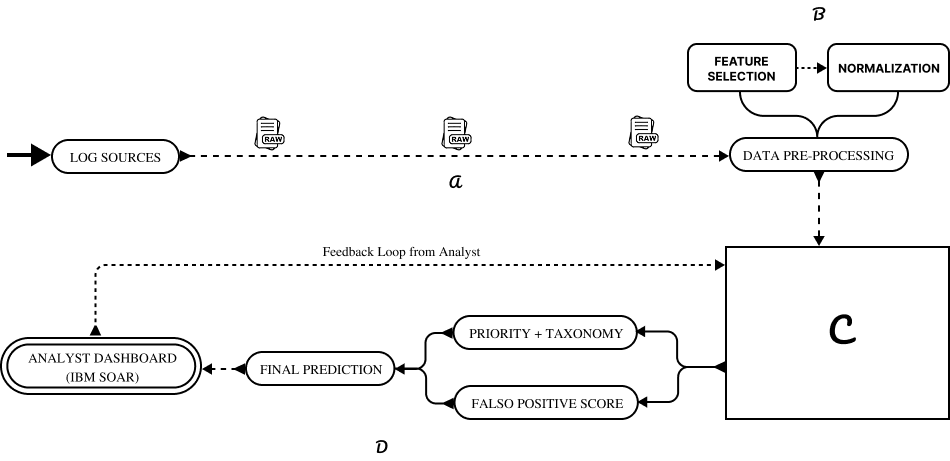
\includegraphics[width=\textwidth]{ch3/assets/general_solution_pipeline.png}
    \caption{General Pipeline for all Three Solutions}
    \label{fig:general_solution_pipeline}
\end{figure}

This pipeline remains largely the same across all solutions, with the exception of section \texttt{C}, where the machine learning model varies depending on the solution. 
While the overall structure of the pipeline is consistent, the type of model used in section \texttt{C} determines the specific prediction process and outputs.

To interpret the figure, a reader should understand the following stages in the pipeline:
\begin{itemize}
    \item \textbf{Section A:} Raw security alerts are collected from various sources, such as SIEM systems, IDS, and firewalls. The data is then standardized to ensure consistency.
    \item \textbf{Section B:} The collected data undergoes preprocessing, which includes cleaning, normalization, and feature extraction.
    \item \textbf{Section C:} This section involves the machine learning model. The specific model used here varies depending on the solution, and it generates predictions based on the preprocessed data.
    \item \textbf{Section D:} Finally, the predictions are displayed on the IBM SOAR dashboard. Analysts can provide feedback on the predictions, and this feedback is used to improve the model over time.
\end{itemize}

The diagram helps visualize how the raw data moves through the system and how the predictions are continuously refined with feedback from the analysts.

\subsubsection{Random Forest with Reinforcement Learning Feedback Loop}

The first solution proposed in this study is a two-layered machine learning system that integrates a Random Forest model with a Reinforcement Learning feedback loop. 

This solution addresses the problem using a pre-trained RF model on historical data combined with an RL model that refines predictions based on analyst feedback.
This integration of \underline{RF with RL} contributes to the model's adaptability, making it highly responsive to new threats.

\paragraph{Design} 

The RF model serves as the decision-making core, trained on a historical dataset of security alerts to classify incoming alerts by taxonomy and priority—\hyperref[objective3]{Objective 3}.

While the RF model provides strong initial predictions, it struggles to adapt to new attack vectors not represented in its training data. 
To address this, the RL model enhances the predictions made by the RF model and evaluates alerts as false positives or true positives, using feedback from security analysts.

The \underline{implementation complexity} of this solution is considered \underline{moderate}, as it does not involve highly intricate algorithms or architectures. 
However, the necessity to implement and integrate two distinct models—a RF for initial predictions and a RL model for feedback-driven refinement—adds an additional layer of complexity. 

Key features of this solution include:
\begin{itemize}
    \item The RL model adjusts its parameters through a continuous feedback loop, improving classification and generating confidence scores.
    \item This dynamic learning process ensures the system is able to handle both \underline{\texttt{cold start}} issues effectively (thanks to the pre-trained RF model) and false positives in real-time.
    \item The system's \underline{adaptability} to new threats is \underline{high via the RL model} and helps manage false positives by learning patterns of false positives or true positives, refining its algorithms, and potentially reducing analysts' workloads.
    \item Designed to efficiently manage and analyze real-time alerts generated from a diverse range of log sources—\hyperref[objective4]{Objective 4}.
\end{itemize}

The \underline{interpretability} of this solution is considered \underline{moderate} due to the significant role played by AI in its decision-making processes. 
The RF model, being a supervised learning algorithm, provides a level of transparency as its outputs can be traced back to the quality and features of the historical dataset used for training. 

However, integrating RL complicates interpretability. RL's iterative feedback and rewards lead to less transparent reasoning, making analyzing and communicating insights challenging.

Integrating this solution with \underline{IBM SOAR} is relatively \underline{easy and straightforward}. 
By relying on the API endpoints provided by this solution, IBM SOAR can seamlessly communicate with the solution platform.
This is vital for enhancing the overall effectiveness of the solution—\hyperref[objective5]{Objective 5}. 

IBM SOAR provides customization of dashboards presented to analysts, enabling:

\begin{itemize}
    \item Creation of custom fields where analysts can view the solution's outputs and mark them as correct or incorrect.
    \item Feedback from analysts, which is crucial for the RL model to learn from mistakes and improve over time.
\end{itemize}

This feedback loop supports continuous refinement and enhances accuracy for future predictions. 
Overall, this strategy leverages the strengths of supervised and reinforcement learning to create a robust solution for security alert triage. 
It enhances operational efficiency and threat response capabilities by:

\begin{itemize}
    \item Minimizing false positives through continuous improvement.
    \item Allowing integration with IBM SOAR to evaluate and test the solution's effectiveness in categorizing alerts and minimizing false positives—\hyperref[objective6]{Objective 6}.
\end{itemize}

\paragraph{Pipeline} 

The illustration in Figure~\ref{fig:solution1_c} corresponds to section \texttt{C} of the general pipeline in Figure~\ref{fig:general_solution_pipeline}. 

\begin{figure}[h!]
    \centering
    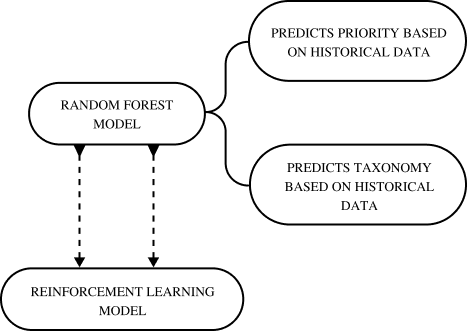
\includegraphics[width=0.5\textwidth]{ch3/assets/solution1_C.png}
    \caption{Part C of the General Pipeline for the Random Forest with Reinforcement Learning Feedback Loop Solution}
    \label{fig:solution1_c}
\end{figure}

This figure provides a detailed representation of the machine learning model's specific implementation for this solution. 

It elaborates on the processes and components that occur within section \texttt{C}, as outlined in the general pipeline, showcasing the unique aspects of this solution's approach to data processing and prediction generation.

\subsubsection{End-to-End Deep Learning Classifier with Feature Fusion}
The second solution in this study employs a deep neural network (DNN) model trained end-to-end on labeled security alert data, based on historical alerts dataset—\hyperref[objective3]{Objective 3}. 

Unlike solution one, which uses a pre-trained RF model, this approach processes raw SIEM logs, analyst comments, and metadata through the DNN's attention layers to automatically extract features and classify data, eliminating the need for manual feature engineering.

While solution one adapts to new threats with a reinforcement learning feedback loop, solution two relies solely on the DNN model, necessitating training on a comprehensive dataset before deployment. 
The DNN excels in complex feature extraction environments but requires periodic retraining based on analyst feedback.

\paragraph{Design}

In this solution, the \underline{DNN model} processes raw security alert data directly, leveraging attention mechanisms to identify and prioritize critical features like alert descriptions, origins, and metadata. 

The attention layers enhance the model's ability to focus on relevant patterns, improving classification accuracy and adaptability. 

By automating feature extraction, this approach streamlines the pipeline, reducing dependency on domain-specific preprocessing techniques.

Key aspects of this solution are:
\begin{itemize}
    \item The DNN model takes in raw security alert data, which is vectorized, and outputs predictions on alert taxonomy, priority, false positive status, and confidence score.
    \item The DNN model's \underline{adaptability} is \underline{moderate} and depends on the training data's quality and diversity. Once trained, it performs well on known data but is less responsive to new attack patterns unless retrained with fresh data.
    \item Solution two faces challenges with cold start problems, as the DNN model requires a substantial amount of labeled training data before it can begin making accurate predictions. Unlike solution one, which benefits from the pre-trained RF model, this solution requires extensive training before it can function effectively.
    \item Engineered to effectively process and evaluate real-time alerts originating from a wide variety of log sources—\hyperref[objective4]{Objective 4}.
\end{itemize}

The \underline{implementation complexity} of solution two is considered \underline{high} due to the extensive computational resources required to train the DNN model. 
Training a deep neural network, especially one that handles raw alert data with attention mechanisms, demands significant time and resources, making it more complex to implement.

The \underline{interpretability} of the solution is \underline{low}, primarily because the DNN model operates as a "black box". 
While it offers powerful predictions, the model's inner workings are difficult to explain, particularly when attention layers are involved, making it harder to interpret why certain predictions were made.

This solution integrates with IBM SOAR for real-time feedback and performance evaluation—\hyperref[objective5]{Objective 5}, allowing analysts to review predictions and provide feedback, which is subsequently used for periodic retraining to assess and validate the solution's capability in classifying alerts and reducing the occurrence of false positives—\hyperref[objective6]{Objective 6}.

\subsubsection{Rule-Augmented Decision Tree with Feedback Aggregation}

The third solution proposed in this study integrates static expert rules with a lightweight \underline{\gls{DTC}}. 
This hybrid system uses a rule engine to pre-filter known benign or critical alert patterns before passing any unknown or ambiguous cases to the \underline{\gls{DTM}}. 

The rules provide initial filtering for quick decisions on clear alerts. For complex cases, the DTC predicts based on available data. 
Feedback is reviewed in batches, enabling periodic updates to the rule base and retraining of the decision tree.

\paragraph{Design}

This solution combines the benefits of domain-specific rules with machine learning.
It starts with a rule engine that quickly processes alerts based on known patterns, tagging them as benign or critical and minimizing the need for further analysis. 
This approach is efficient in environments with well-defined, static patterns. 
This solution will be designed to ingest data from a variety of log sources, including SIEM systems and other security tools—\hyperref[objective4]{Objective 4}.

The rule engine will preprocess and filter alerts from these sources, leveraging predefined rules to handle known patterns efficiently, while less adaptive, predefined rules to filter known benign patterns, ensuring a baseline reduction in false positives. 

For alerts that don't fit predefined rules, the DTC classifies them using features from raw data, allowing the system to manage both known and unknown patterns while balancing interpretability and accuracy. 

The DTC works with a clean, segmented dataset to differentiate between alerts that match known patterns and those requiring further analysis—\hyperref[objective3]{Objective 3}.

Key features of this solution include:
\begin{itemize}
    \item The rule engine filters known benign or critical patterns before passing uncertain alerts to the DTC. This approach reduces the overall processing time and helps prioritize more ambiguous cases.
    \item \underline{Feedback} is logged and applied asynchronously, meaning that the system doesn't update in real-time. Instead, the rule base is updated, and the decision tree is retrained on a \underline{periodic basis (e.g., weekly)}. This ensures that the system evolves over time but does not immediately adjust to new threats in real-time.
    \item The system's ability to \underline{handle new and evolving threats} is \underline{low}, as it depends on manually updating the rule base to address new threats.
    \item \underline{\textit{Cold start}} handling is excellent because the rules-based filtering system can operate immediately without requiring training, and the DTC is lightweight enough to be quickly deployed after the initial setup.
\end{itemize}

The \underline{implementation complexity} of this solution is \underline{low}, as it uses well-understood decision tree models and a simple rule engine. 
This makes it relatively \underline{easy to implement} when compared to the other solutions. 
However, the trade-off is that the DTC may not be as powerful as deep learning-based models or even RL models when dealing with complex, high-dimensional data.

The \underline{interpretability} of this solution is considered \underline{high}. 
Both the rule engine and the decision tree are inherently interpretable, allowing analysts to understand the reasoning behind the classifications. 
This makes it particularly useful in environments where auditability and transparency are important. 
However, the model's inability to \underline{adapt} in real-time can make it \underline{less suitable} for \underline{rapidly evolving attack patterns}.

Integrating this solution with \underline{IBM SOAR} is \underline{straightforward}, allowing for seamless communication between the alert system and the dashboard used by analysts. 
Alerts classified by the rule engine and decision tree are sent to the IBM SOAR dashboard, where analysts can review predictions and provide feedback—\hyperref[objective5]{Objective 5}.
The feedback is stored and reviewed periodically to refine the rules and retrain the decision tree. 

\subsubsection{Architecture}

The diagram in Figure~\ref{fig:architecture} illustrates the architecture for all solutions.

\begin{figure}[h!]
    \centering
    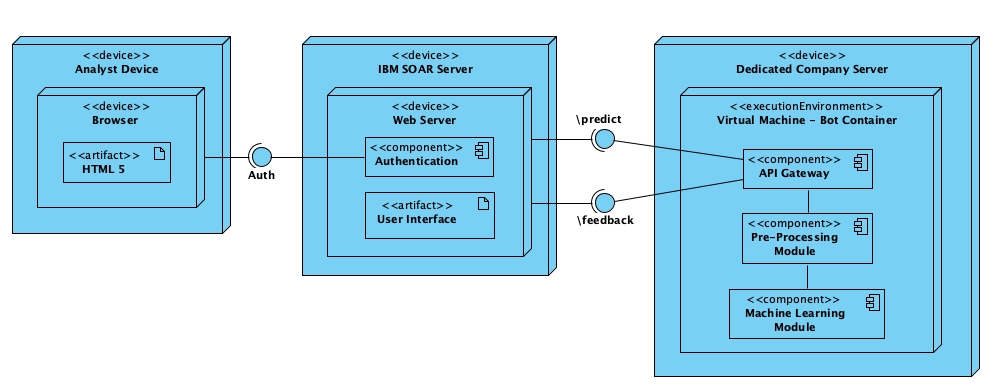
\includegraphics[width=\textwidth]{ch3/assets/archquiteture.png}
    \caption{Architecture of the Random Forest with Reinforcement Learning Feedback Loop Solution}
    \label{fig:architecture}
\end{figure}

It's organized into three major sections:
\begin{enumerate}
    \item \textbf{Analyst Device}: This device acts as the point of interaction where security analysts review and manage alerts. Represents the user interface. The analyst logs into the system through the \textbf{Authentication} component, enabling access to the dashboard.
    
    \item \textbf{IBM SOAR Server}: The IBM SOAR Server is the central system for managing security alerts. The server sends requests to the \textbf{Bot Container} through the \texttt{\textbackslash predict} endpoint, triggering the alert classification process. Once the alert is processed, the \texttt{\textbackslash feedback} endpoint is used to receive the analyst's input for further training of the RL model.
    
    \item \textbf{Dedicated Company Server}: The \textbf{Dedicated Company Server} hosts the \textbf{Bot Container}, which is deployed on a \textbf{Virtual Machine (VM)}. This container is responsible for the core functionality of the solution, consisting of three main components:
    \begin{itemize}
        \item \textbf{API Gateway}: This component serves as the entry point for receiving requests from the IBM SOAR Server and handling communication between the components inside the bot container. It processes the incoming alert data and forwards it to the appropriate modules.
        \item \textbf{Pre-Processing Module}: This module cleans and prepares the incoming alert data, extracting features and transforming them into a suitable format for the model.
        \item \textbf{Machine Learning Module}: The \textbf{Machine Learning Module} applies the \gls{RF} model to classify the alert. These predictions are then further refined through the \gls{RL} model.
    \end{itemize}
\end{enumerate}

This architecture is designed to be modular and scalable, allowing for easy integration with existing systems and the ability to adapt to evolving security threats.


%----------------------------------------------------------------------------------------

\subsection{Comparative Analysis}
Table~\ref{tab:solution_comparison} presents a comparison of the three proposed approaches based on key evaluation criteria. 
The goal is to assess their suitability in the context of a real-world SOC environment, taking into consideration implementation complexity, adaptability, performance, interpretability, and integration potential.

\captionsetup[table]{font=small} % Set the caption font size
\scriptsize % Reduce the font size for the table content
\begin{longtable}{@{}P{3cm}P{3cm}P{4cm}P{4cm}@{}}
    \caption{Comparison of Proposed Solutions}
    \label{tab:solution_comparison} \\
    \toprule
    \textbf{Criteria} & \textbf{\gls{RF} + \gls{RL}} & \textbf{\gls{DNN}} & \textbf{Rules + Decision Tree} \\
    \midrule
    \endfirsthead

    \toprule
    \textbf{Criteria} & \textbf{\gls{RF} + \gls{RL}} & \textbf{\gls{DNN}} & \textbf{Rules + Decision Tree} \\
    \midrule
    \endhead

    \bottomrule
    \endfoot

    \bottomrule
    \endlastfoot

    Architecture Type & \gls{RF} + \gls{RL} (Two-layer) & \gls{DNN} & Rule-based + Decision Tree \\
    \vspace{0.2cm}
    Implementation Complexity & Moderate & High & Low \\
    \vspace{0.2cm}
    Adaptability to New Threats & High (via \gls{RL}) & Moderate (via retraining) & Low (manual updates) \\
    \vspace{0.2cm}
    Learning from Feedback & Online (via \gls{RL}) & Periodic retraining & Batch/manual integration \\
    \vspace{0.2cm}
    Cold Start Handling & Excellent (\gls{RF} pre-trained) & Poor & Excellent (rules pre-set) \\
    \vspace{0.2cm}
    Interpretability & Moderate & Low & High \\
    \vspace{0.2cm}
    Scalability & High & High & Moderate \\
    \vspace{0.2cm}
    Integration with SIEM (IBM SOAR) & Easy & Easy & Easy \\
    \vspace{0.2cm}
    False Positive Reduction & Adaptive (confidence scoring) & Model confidence only & Rigid (rule-defined) \\
    \vspace{0.2cm}
    Performance in Evolving Scenarios & High & Moderate & Low \\
    
\end{longtable}

\normalsize

% \textbf{Solution 1} combines RF with RL, offering a highly adaptable system that continuously improves its performance over time. 
% The integration of RF for initial predictions and RL for feedback-based adjustments allows the system to react to evolving cybersecurity threats.

% \begin{itemize}
%     \item The implementation complexity is moderate, as integrating two models (RF and RL) requires careful setup but remains manageable with existing frameworks like scikit-learn and RLlib.
%     \item High adaptability, as the RL model continuously adjusts based on analyst feedback. The system can handle new attack patterns without requiring manual updates, making it effective in dynamic environments.
%     \item This solution uses online learning through the RL feedback loop, which means feedback from analysts is immediately integrated into the model, refining its predictions in real-time.
%     \item Excellent cold start handling, thanks to the pre-trained RF model. This allows the system to make predictions right away, with the RL model improving its performance gradually over time.
%     \item Moderate interpretability due to the transparency of the RF model, but the integration of RL adds complexity, making it harder to explain the decision-making process.
%     \item High performance in evolving scenarios, as the RL model adapts in real-time to new data, making it well-suited for fast-changing threat landscapes.
% \end{itemize}

% \textbf{Solution 2} uses a DNN that processes raw alert data through attention mechanisms to automatically extract features and classify alerts. 
% Unlike \textbf{Solution 1}, it doesn't use RL for real-time feedback but relies on periodic retraining to improve performance.

% \begin{itemize}
%     \item High implementation complexity because training a DNN requires substantial computational resources and time, especially when handling raw data with attention mechanisms. This makes it more complex to implement compared to \textbf{Solution 1}.
%     \item Moderate adaptability. The DNN model learns from feedback, but it does so through periodic retraining. It doesn't adjust in real-time like \textbf{Solution 1}, making it less responsive to new threats immediately after they emerge.
%     \item Feedback is applied during periodic retraining. This means the model improves over time but is slower to adapt compared to \textbf{Solution 1}, which has real-time learning through RL.
%     \item Poor cold start handling. The DNN model requires a significant amount of labeled data to be trained before it can start making reliable predictions. It cannot provide immediate predictions like \textbf{Solution 1}.
%     \item Low interpretability. DNN models are often considered “black boxes,” making it difficult to explain how certain predictions were made, especially when attention mechanisms are involved.
%     \item Moderate performance. While the DNN is effective on known data, it needs retraining to adjust to new, unseen patterns, making it less suited for dynamic cybersecurity environments compared to \textbf{Solution 1}.
% \end{itemize}

% \textbf{Solution 3} integrates static expert rules with a lightweight DTC. 
% The rule engine filters known patterns, while the DTC handles ambiguous or unknown cases. 
% Feedback is aggregated and applied periodically to retrain the decision tree and refine the rules.

% \begin{itemize}
%     \item Low implementation complexity. The system is built with simple decision tree algorithms and rule-based filtering, making it easier to implement compared to the more complex \textbf{Solution 1} and \textbf{Solution 2}.
%     \item Low adaptability. The system relies on manual updates to the rules base to address new attack vectors. It is not capable of real-time adjustments like \textbf{Solution 1}.
%     \item Feedback is applied asynchronously. The system doesn't adjust in real-time but instead uses periodic feedback to update the rules and retrain the decision tree. This makes it slower to improve and adapt to changing threats.
%     \item Excellent cold start handling. The rules-based system can immediately classify alerts based on predefined patterns, and the DTC can be deployed quickly without extensive data preparation.
%     \item High interpretability. Both the rule engine and DTC are transparent, allowing security analysts to easily understand the rationale behind decisions. This is a major advantage in environments that require auditing and explainability.
%     \item Low performance in evolving scenarios. The system relies on static rules, which require manual updates to accommodate new threats. It is less flexible than \textbf{Solution 1} or \textbf{Solution 2}, making it less effective in rapidly changing cybersecurity environments.
% \end{itemize}

% \subsubsection{Overall Evaluation}

Solution 1 is optimal because it offers adaptability, scalability, and real-time learning. 
Integrating RF with RL continuously adapts to new threats through real-time feedback, making it highly effective in dynamic cybersecurity environments.

Solution 2 excels in feature extraction using DNN but lacks immediate adaptability. 
It requires periodic retraining, making it less responsive to evolving threats than Solution 1.

Solution 3, while simple and interpretable, is not adaptable. 
It relies on static rules and manual updates, making it less suitable for fast-changing threat landscapes.

In conclusion, Solution 1 is the best option for real-time alert classification and long-term adaptability in a SOC environment.

\section{Proof of Concept}
This section presents the practical implementation of the proposed solution, including the setup of the test environment, preparation of the dataset, and execution of the ML models. It aims to demonstrate the feasibility and performance of the selected approach under realistic conditions.

\subsection{Data Processing}
This section outlines the process of refining the raw data, corresponding to phase B in the solution pipeline.

As previously mentioned, Solution One was the best choice among the three alternatives.

To implement this solution effectively, ArtResilia provided a dataset of security alerts generated by its SOC. 

This dataset, covering the period from February 9, 2022, to January 31, 2025, encompasses various alerts categorized by attributes, such as priority and taxonomy. 
The primary goal of the data processing phase was to prepare this raw data for training ML models to predict the priority and taxonomy of alerts based on the textual descriptions associated with each alert.

\begin{figure}[h!]
    \centering
    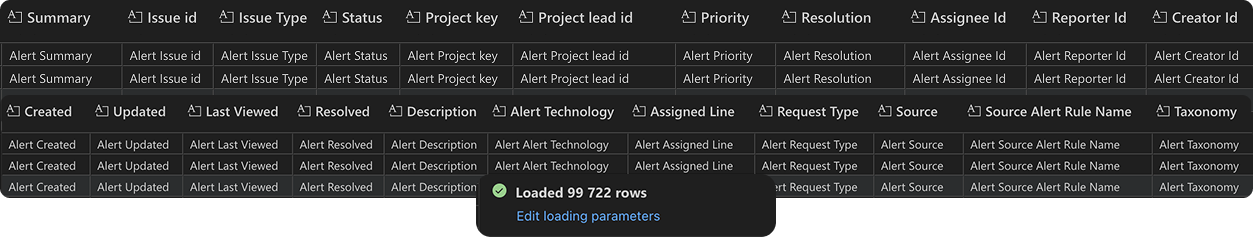
\includegraphics[width=\textwidth]{ch3/assets/dataset_original.png}
    \caption{Original Dataset Before Preprocessing}
    \label{fig:dataset_original}
\end{figure}

Figure~\ref{fig:dataset_original} illustrates the original dataset before preprocessing.
The dataset\footnote{For privacy reasons, the actual data has been censored or altered to ensure confidentiality.} contains 99,722 rows, each representing a security alert.

To prepare the data for training ML models, several key preprocessing steps were performed:

\paragraph{First Step}
Rows missing data in "Priority" or "Taxonomy" were removed, retaining only the essential columns: "Description", "Priority", and "Taxonomy". 
These columns provide the text for training and the target labels.

Listing~\ref{lst:first_preprocessing} shows the Python code snippet used for this initial preprocessing step.

\vspace{0.2cm}
\noindent
\begin{minipage}{\linewidth}
\begin{minted}{python}
df = df[(df['Source'] != 'Other') & (df['Source Alert Rule Name'].notna())]
required_columns = ["Description", "Priority", "Taxonomy"]
df = df[required_columns]
df = df.dropna(subset=required_columns)
\end{minted}
\captionof{listing}{Python Code Snippet for the First Part of Preprocessing the Dataset.}
\label{lst:first_preprocessing}
\end{minipage}
\vspace{0.1cm}

\paragraph{Second Step}
Alerts with a Priority of "P4" or a Taxonomy labeled as "Other" were also excluded as these were deemed less relevant for the model's prediction task. 
To address class imbalance in the Taxonomy column, random oversampling was performed. 
This involved ensuring that smaller categories had enough examples for the model by duplicating instances from underrepresented taxonomies until they matched the size of the largest category.

Listing~\ref{lst:second_preprocessing} provides the Python code snippet used for the second preprocessing step, which includes filtering and oversampling to address class imbalance in the dataset. 

\vspace{0.2cm}
\noindent
\begin{minipage}{\linewidth}
\begin{minted}{python}
df = df[(df["Priority"] != "P4") & (df["Taxonomy"].str.lower() != "other")]
taxonomy_counts = df["Taxonomy"].value_counts()
max_len = taxonomy_counts.max()
oversampled_dfs = []
for tax, count in taxonomy_counts.items():
    sub_df = df[df["Taxonomy"] == tax]
    if count < max_len:
        diff = max_len - count
        extra_rows = sub_df.sample(n=diff, replace=True, random_state=42)
        sub_df = pd.concat([sub_df, extra_rows], ignore_index=True)
    oversampled_dfs.append(sub_df)
df = pd.concat(oversampled_dfs, ignore_index=True)
\end{minted}
\captionof{listing}{Python Code Snippet for the Second Part of Preprocessing the Dataset.}
\label{lst:second_preprocessing}
\end{minipage}
\vspace{0.1cm}

By applying the preprocessing code above from steps one and two, the dataset was reduced from its original 99,722 rows, representing security alerts, to approximately 81,732 rows.
However, after the oversampling process, the dataset was expanded to around 173,637 rows, ensuring a balanced representation of all taxonomies.

\paragraph{Third Step}

The "Description" column, which contains raw text data, was also cleaned. 
Unnecessary formatting was removed as well as special characters, and irrelevant sections (such as URLs and IBM SOAR links). 
It also handled tasks like stripping extra whitespace and removing HTML tags, ensuring the text was in a consistent and usable format for the machine learning pipeline.

Listing~\ref{lst:third_preprocessing} shows the Python code snippet used for this third preprocessing step.

\vspace{0.2cm}
\noindent
\begin{minipage}{\linewidth}
\begin{minted}{python}
df["Description"] = df["Description"].progress_apply(clean_text)
\end{minted}
\captionof{listing}{Python Code Snippet for the Third Part of Preprocessing the Dataset.}
\label{lst:third_preprocessing}
\end{minipage}
\vspace{0.1cm}

The code snippet presented above applies the \texttt{clean\_text} function uniformly to all entries within the "Description" column of the dataset, ensuring consistent preprocessing of textual data for subsequent machine learning tasks.

The rules defined for normalizing the description text will be detailed in the next section, where the \texttt{clean\_text} function is explained.

\paragraph{Fourth Step}

Finally, the "Priority" and "Taxonomy" labels were stripped of any leading or trailing spaces to ensure consistency in the dataset. 

Listing~\ref{lst:fourth_preprocessing} shows the Python code snippet used for this final preprocessing step.

\vspace{0.2cm}
\noindent
\begin{minipage}{\linewidth}
\begin{minted}{python}
df["Priority"] = df["Priority"].astype(str).str.strip()
df["Taxonomy"] = df["Taxonomy"].astype(str).str.strip()
\end{minted}
\captionof{listing}{Python Code Snippet for the Fourth Part of Preprocessing the Dataset.}
\label{lst:fourth_preprocessing}
\end{minipage}
\vspace{0.1cm}

These preprocessing steps ensure that the dataset is clean, balanced, and properly formatted, making it ready for use in the ML models. 
The combination of filtering, oversampling, text cleaning, and label processing prepares the data for training while addressing potential issues such as class imbalance and noisy raw data.

\begin{figure}[h!]
    \centering
    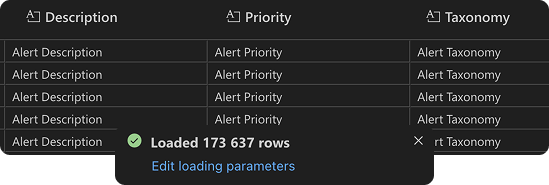
\includegraphics[width=\textwidth]{ch3/assets/dataset_processed.png}
    \caption{Original Dataset After Preprocessing}
    \label{fig:dataset_processed}
\end{figure}

Figure~\ref{fig:dataset_processed} illustrates the dataset\footnotemark[\value{footnote}] after preprocessing, showcasing the difference between the original and processed versions.

\subsection{Data Normalization}
Data normalization typically refers to the process of transforming data into a common scale to improve the performance and accuracy of machine learning models. 

In this project, normalization was applied specifically to the "Description" column, which contains the raw text data. 

This is crucial, as natural language data can contain noise, irrelevant characters, and inconsistencies that can negatively impact model training and performance. 

Unlike the Priority and Taxonomy columns, which are already in categorical formats suitable for ML models, the Description column required more extensive processing to make it usable for training.

As stated in the previous section, the normalization process was performed using a function called \texttt{clean\_text}, which was designed to normalize the raw text in the Description column. 
This function specifically targets common issues in textual data, such as extraneous formatting, unwanted characters, and irrelevant content.

\begin{figure}[h!]
    \centering
    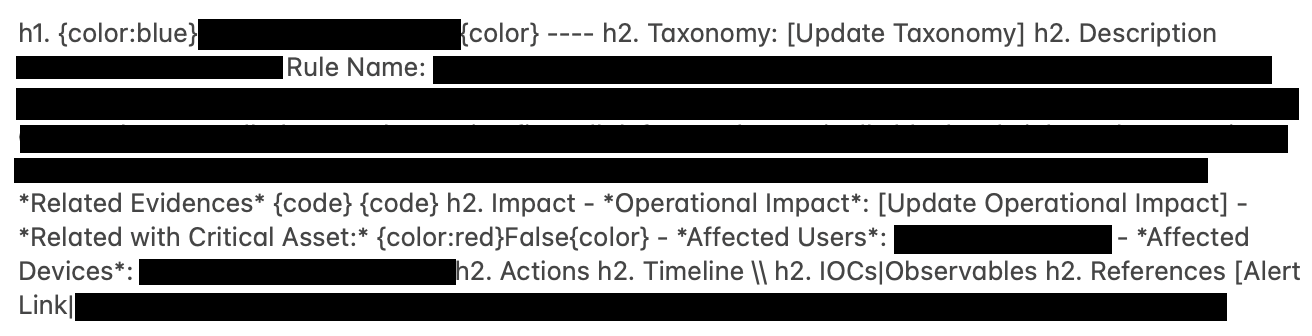
\includegraphics[width=\textwidth]{ch3/assets/redacted_description_text.png}
    \caption{Redacted Description Text}
    \label{fig:redacted_description_text}
\end{figure}

Figure~\ref{fig:redacted_description_text} presents a redacted\footnote{For privacy reasons, the actual data has been censored or altered to ensure confidentiality.} visualization that exemplifies the typical format of a description text.
The formatting of this description may differ based on the source of the alert, highlighting the diverse origins and structures of the data. 
To address these variations, the \texttt{clean\_text} function was created to standardize the presentation of the text data, ensuring it remains consistent regardless of its source.

The \texttt{clean\_text} function performs several key operations:

\begin{itemize}
    \item \textbf{Extract Relevant Content:} Identifies and retains the "Description" section, removing irrelevant sections like "Taxonomy" or "References" if present.
    \item \textbf{Remove Unwanted Characters:} Cleans special symbols, color tags, code markers, HTML tags, and URLs to retain only meaningful content.
    \item \textbf{Text Cleaning:} Strips extra spaces, removes irrelevant phrases (e.g., "action:" or "related evidences:"), and ensures consistent formatting.
    \item \textbf{Handle Rule Name:} Captures and formats rule names with associated narratives as \texttt{<Rule Name> - <Narrative>} for clarity.
    \item \textbf{Final Output:} Returns a cleaned, normalized description.
\end{itemize}

By applying a normalizing function to the Description column helps achieve consistency and reduce noise in the training text data.
The Priority and Taxonomy columns did not require the same normalization process, as they are categorical and do not need extensive text processing.

\subsection{Dataset Division}
Dataset Division refers to how the dataset is split into subsets used for training, validation, and testing. 

This division is crucial because it allows the model to be trained on one subset of the data while ensuring that the model's performance is evaluated on unseen data. 

This prevents overfitting, where the model performs well on training data but fails to generalize to new, unseen data. 

Similarly, proper dataset division also avoids underfitting, where the model might not learn enough from the training data to perform well.
\clearpage
In ML, the dataset is typically divided into three parts:
\begin{itemize}
    \item \textbf{Training Set:} Used to train the model.
    \item \textbf{Validation Set:} Used to tune the model's hyperparameters and prevent overfitting during training.
    \item \textbf{Test Set:} Used to evaluate the final model's performance after training is complete.
\end{itemize}

In this project, the dataset was divided as follows:

\begin{itemize}
    \item \textbf{Training and Test Split:} The data was split into 70\% for training and 30\% for testing. This ratio strikes a balance between providing enough data for the model to learn from, while still maintaining a sufficient amount of data to test its generalization ability. This approach was chosen to maximize the model's ability to generalize to unseen data while preventing overfitting.
\end{itemize}

\vspace{0.2cm}
\noindent
\begin{minipage}{\linewidth}
\begin{minted}{python}
X_train, X_test, Y_train, Y_test = train_test_split(X, Y, test_size=0.3, random_state=42, stratify=stratify_labels)
\end{minted}
\captionof{listing}{Splitting Dataset.}
\label{lst:dataset_split}
\end{minipage}
\vspace{0.1cm}

\begin{itemize}
    \item \textbf{Stratified Sampling:} The split was performed using stratified sampling, ensuring that the proportion of each class in Priority and Taxonomy was maintained across the training and test sets. This helps avoid bias in the dataset and ensures that both the training and test sets have representative distributions of all classes.
\end{itemize}

\vspace{0.2cm}
\noindent
\begin{minipage}{\linewidth}
\begin{minted}{python}
stratify_labels = [tuple(row) for row in Y]
X_train, X_test, Y_train, Y_test = train_test_split(X, Y, test_size=0.3, random_state=42, stratify=stratify_labels)
\end{minted}
\captionof{listing}{Stratified Sampling.}
\label{lst:stratified_sampling}
\end{minipage}
\vspace{0.1cm}

This stratified split is particularly important for imbalanced datasets, as it ensures that each class is proportionally represented in both the training and testing subsets, thereby improving the model's ability to generalize and minimizing bias toward the majority class.

\begin{itemize}
    \item \textbf{Test Set}: The 30\% test set was kept completely separate from the training process, ensuring that the model's performance could be assessed on data it had never seen before. This provides an unbiased evaluation of the model's accuracy and generalization capabilities.
\end{itemize}

By properly dividing the dataset, this approach ensures that the model is trained on a representative subset of data, can be fine-tuned using the validation set, and is evaluated fairly on the test set. 
This helps in achieving a balance between training the model effectively and ensuring generalization without overfitting or underfitting.

\subsection{Machine Learning Model Development}
This section describes the implementation of the RF model and the RL feedback loop, explaining how these models were integrated to complement each other and enhance prediction accuracy in the system.

\subsubsection{Random Forest Model Implementation}

The \textbf{RF model} is implemented using scikit-learn's \textbf{RandomForestClassifier}. 
It is employed as the core decision-making component in the system, trained to predict two target variables: \textbf{priority} and \textbf{taxonomy} of security alerts. 
To handle these \textbf{multi-output targets}, \textbf{MultiOutputClassifier} is used, which allows the model to make predictions on both target variables simultaneously.

The first step in implementing the \textbf{RF model} is to transform the raw textual data in the \textbf{Description} column into numerical features. 
This is achieved using \textbf{SentenceBertVectorizer}, a tool that leverages the \textbf{Sentence-BERT model} to generate embeddings from the alert descriptions. 
These embeddings capture the \textbf{semantic meaning} of the descriptions, which is crucial for the model to make accurate predictions.

\vspace{0.2cm}
\noindent
\begin{minipage}{\linewidth}
\begin{minted}{python}
vectorizer = SentenceBertVectorizer(model_name="paraphrase-MiniLM-L6-v2")
X = vectorizer.fit_transform(df["Description"])
\end{minted}
\captionof{listing}{Vectorizing Text Data.}
\label{lst:vectorizing_text_data}
\end{minipage}
\vspace{0.1cm}

Once the text data is vectorized, the target labels (Priority and Taxonomy) are encoded using LabelEncoder. 
This step converts the categorical labels into numeric form, making them suitable for input into the RF model.

\vspace{0.2cm}
\noindent
\begin{minipage}{\linewidth}
\begin{minted}{python}
# Encode targets for Priority and Taxonomy
le_priority = LabelEncoder()
le_taxonomy = LabelEncoder()
y_priority = le_priority.fit_transform(df["Priority"])
y_taxonomy = le_taxonomy.fit_transform(df["Taxonomy"])

# Combine the targets into a 2D array
Y = np.column_stack((y_priority, y_taxonomy))
\end{minted}
\captionof{listing}{Encoding Target Labels.}
\label{lst:encoding_target_labels}
\end{minipage}
\vspace{0.1cm}

Next, the dataset is split into training and testing sets using train\_test\_split from scikit-learn. 
This ensures that the model is trained on one subset of data and evaluated on another, providing an unbiased assessment of its performance.

\vspace{0.2cm}
\noindent
\begin{minipage}{\linewidth}
\begin{minted}{python}
# Split the data into training and testing sets
X_train, X_test, Y_train, Y_test = train_test_split(X, Y, test_size=0.3, random_state=42, stratify=Y)
\end{minted}
\captionof{listing}{Splitting the Dataset.}
\label{lst:splitting_dataset}
\end{minipage}
\vspace{0.1cm}

After splitting the data, the RandomForestClassifier is initialized and wrapped with MultiOutputClassifier to handle the multi-output prediction task. 
The model is trained on the training data and evaluated on the test set. 

\vspace{0.2cm}
\noindent
\begin{minipage}{\linewidth}
\begin{minted}{python}
# Train a MultiOutputClassifier using RandomForest
base_rf = RandomForestClassifier(n_estimators=500, random_state=42, max_depth=40, min_samples_split=10)
multi_rf = MultiOutputClassifier(base_rf)
multi_rf.fit(X_train, Y_train)
\end{minted}
\captionof{listing}{Training the Random Forest Model.}
\label{lst:training_rf_model}
\end{minipage}
\vspace{0.1cm}

\subsubsection{Reinforcement Learning Model Implementation}

While the RF model is capable of making initial predictions, it requires further refinement to adapt to new or unseen threats. 
This is where the RL model comes in. The RL model is designed to improve predictions by incorporating feedback from security analysts.

The RL model is built using the Proximal Policy Optimization (PPO) algorithm from Stable Baselines3, a popular library for RL. 
The model's role is to adjust the predictions made by the RF model based on feedback received from analysts. 

At the core of this RL model is a reward function that is based on whether the model's predictions are correct, focusing on both false positive (FP) and true positive (TP) predictions for taxonomy and priority. 
The reward function is designed to penalize incorrect predictions and reward correct ones, with particular weight given to more critical mistakes.

\paragraph{False Positive (FP) Evaluation}
The third element of the action vector represents the \textbf{RL model's FP prediction}. 

A positive reward is given if the model's FP prediction matches the ground truth, while a penalty is applied if the prediction is incorrect.

\[
R_{\text{FP}} = 
\begin{cases} 
+ w_{\text{tp}} \cdot \text{confidence} & \text{if FP prediction is correct} \\
- w_{\text{fn}} & \text{if predicted FP but true TP} \\
- w_{\text{fp}} & \text{if predicted TP but true FP} \\
\end{cases}
\label{eq:fp_reward}
\]

\paragraph{Priority and Taxonomy Classification}
The \textbf{priority} and \textbf{taxonomy} predictions are compared to the true values. A penalty is applied if either the priority or taxonomy prediction is incorrect.

\[
R_{\text{error}} = \alpha \cdot \text{priority\_error\_indicator} + \beta \cdot \text{taxonomy\_error\_indicator}
\label{eq:error_penalty}
\]

\paragraph{Final Reward}
The final reward is the sum of the FP evaluation and the error penalties for priority and taxonomy:

\[
R = R_{\text{FP}} - R_{\text{error}}
\label{eq:final_reward}
\]

Where:
\begin{itemize}
    \item \( w_{\text{tp}} \) is the weight for true positives,
    \item \( w_{\text{fn}} \) and \( w_{\text{fp}} \) are penalties for false negatives and false positives, respectively,
    \item \( \alpha \) and \( \beta \) are the penalty weights for priority and taxonomy errors,
    \item \textbf{confidence} is the model’s confidence in its FP prediction,
    \item \textbf{priority\_error\_indicator} and \textbf{taxonomy\_error\_indicator} are binary values indicating whether the respective predictions are correct.
\end{itemize}

This reward function allows the RL model to adjust its predictions based on feedback, ensuring continuous improvement in the model's performance.

The RL agent uses the above reward function to adjust its policy (i.e., how it makes predictions) based on the rewards it receives after each prediction. 
The PPO algorithm ensures that policy updates are stable and efficient, making it well-suited for real-time systems.

To manage computational load during training, the RL model is trained asynchronously using Celery, a distributed task queue. 
Celery ensures that training tasks do not block other system operations, enabling the RL model to be trained in parallel with real-time alert classification.

Here's an example of how the RL training task is defined using Celery:

\vspace{0.2cm}
\noindent
\begin{minipage}{\linewidth}
\begin{minted}{python}
@celery_app.task
def train_rl_agent_task(feedback, model_version):
    dummy_env = RLDummyEnv(observation_dim=386)
    rl_agent = PPO.load(src.config.RL_AGENT_PATH, env=dummy_env)

    model = load_model(model_version)
    result_info = update_rl_agent_with_feedback(feedback, model, rl_agent)
    return result_info
\end{minted}
\captionof{listing}{RL Training Task with Celery.}
\label{lst:rl_training_task}
\end{minipage}
\vspace{0.1cm}

This asynchronous processing model allows the RL agent to continuously improve based on real-time feedback while ensuring that the system remains responsive to new alert data.
Although, for this to happen the RL model need to be trained in a separate process to ensure efficient and uninterrupted training. 
However, this separation means that the most recently trained version of the model is not immediately available to the main process responsible for making predictions. 

To address this, the training process saves the model to persistent storage each time training is completed. 

The main process, whenever it needs to use the RL model, checks if the model has been updated since the last time it was loaded. 
If a newer version is detected, the main process reloads the model, ensuring that it always operates with the most up-to-date version of the RL model.
This approach maintains consistency between training and inference while allowing both processes to function independently.

\subsection{Hyperparameter Tuning}

In the process of model development, hyperparameter tuning was performed for both the \gls{RF} and \gls{RL} models to optimize their performance. 

The primary goal of hyperparameter tuning is to find the best configuration of hyperparameters that allows the models to generalize well to unseen data, reducing the risk of overfitting while maintaining high predictive accuracy.

For the \gls{RF} model, tests were run using a \texttt{GridSearchCV} approach to explore a range of hyperparameters. 
However, after extensive testing, the most effective hyperparameters were identified and are now used in the model's initialization. 

\begin{itemize}
    \item \textbf{Number of estimators (\texttt{n\_estimators})}: Set to 500.
    \item \textbf{Maximum depth (\texttt{max\_depth})}: Set to 40.
    \item \textbf{Minimum samples required to split an internal node (\texttt{min\_samples\_split})}: Set to 10.
    \item \textbf{Minimum samples required at each leaf node (\texttt{min\_samples\_leaf})}: Set to 1.
    \item \textbf{Class weight (\texttt{class\_weight})}: Set to \texttt{'balanced'}.
\end{itemize}

The following code snippet reflects the initialization of the RF model with the chosen hyperparameters:

\vspace{0.2cm}
\noindent
\begin{minipage}{\linewidth}
\begin{minted}{python}
base_rf = RandomForestClassifier(n_estimators=500, random_state=42, 
                                max_depth=40, min_samples_split=10, 
                                min_samples_leaf=1, class_weight='balanced')
multi_rf = MultiOutputClassifier(base_rf)
\end{minted}
\captionof{listing}{Random Forest Model Initialization.}
\label{lst:rf_model_initialization}
\end{minipage}
\vspace{0.1cm}

For the \gls{RL} model, a similar approach was used, but the model's hyperparameters, such as learning rate, batch size, and the number of epochs, were fine-tuned to ensure that the model could learn efficiently from feedback while maintaining stability in training. 
The PPO algorithm was used, which is known for its stability and effectiveness in reinforcement learning tasks. 
The key parameters for the \gls{RL} model include:

\begin{itemize}
    \item \textbf{Learning rate}: Set to 3e-4.
    \item \textbf{Batch size}: Set to 64.
    \item \textbf{Number of epochs}: Set to 4.
    \item \textbf{Gamma}: Set to 0.99.
    \item \textbf{GAE lambda}: Set to 0.9.
    \item \textbf{Entropy coefficient}: Set to 0.01.
\end{itemize}

The \gls{RL} model's training process is designed to adjust its predictions based on the feedback it receives, improving accuracy over time by refining its policy.

Both models underwent comprehensive testing to determine the optimal set of hyperparameters. Ultimately, the configurations used in the models' initialization were found to provide the best balance between performance, accuracy, and generalization.

The finalized hyperparameters are now used in the model pipelines, ensuring efficient training and reliable predictions.

\chapter{Chapter 4}
\label{chap:Chapter4}
\chapter{Conclusion and Future Work}
\label{chap:Chapter5}

\section{Future Work}


%----------------------------------------------------------------------------------------
%	BIBLIOGRAPHY
%----------------------------------------------------------------------------------------

\printbibliography[heading=bibintoc]

%----------------------------------------------------------------------------------------
%	THESIS CONTENT - APPENDICES
%----------------------------------------------------------------------------------------
% Include the appendices of the thesis as separate files from the Appendices folder
% Uncomment the lines as you write the Appendices
% \begin{appendices}

% % Appendix A

\chapter{Appendix Title Here} % Main appendix title

\label{AppendixA} % For referencing this appendix elsewhere, use \ref{AppendixA}

Write your Appendix content here.
% %\input{appendices/appendixB}
% %\input{appendices/appendixC}

% \end{appendices}
%----------------------------------------------------------------------------------------

\end{document}
